\documentclass[11pt]{jsreport}
\usepackage[dvipdfmx]{graphicx}
\usepackage{url}
\usepackage{enumerate}
\usepackage{tabularx}

\makeatletter%% プリアンブルで再定義する際は必須

\def\@makechapterhead#1{\hbox{}%
  \vskip2\Cvs
  {\parindent\z@
%  \raggedright% 左揃え(オリジナルの定義)
  \centering% 中央揃え
%  \raggedleft% 右揃え
  \normalfont\huge\sffamily\gtfamily%% フォントを変更する
  \leavevmode
  \ifnum \c@secnumdepth >\m@ne
    \setlength\@tempdima{\linewidth}%
%%%    \if@mainmatter% ← report クラスの場合この行不要
%    \setbox\z@\hbox{\@chapapp\thechapter\@chappos\hskip1zw}%
%    \addtolength\@tempdima{-\wd\z@}%
%    \unhbox\z@\nobreak
%%%    \fi% ← report クラスの場合この行不要
    \vtop{\hsize\@tempdima\@chapapp\thechapter\@chappos\hskip1zw#1}%
  \else
    #1\relax
  \fi}\nobreak\vskip3\Cvs}
%
\def\@makeschapterhead#1{\hbox{}%
  \vskip2\Cvs
  {\parindent\z@
%  \raggedright% 左揃え(オリジナルの定義)
  \centering% 中央揃え
%  \raggedleft% 右揃え
  \normalfont\huge\sffamily\gtfamily%% フォントを変更する
  \leavevmode
  \setlength\@tempdima{\linewidth}%
  \vtop{\hsize\@tempdima#1}}\vskip3\Cvs}

\makeatother%% プリアンブルで再定義する際は必須

\begin{document}
\pagestyle{empty}

%
% 表紙
%
%近畿大学理工学部情報学科卒業研究報告書表紙
% ver 0.1 2005/11/28 by Toru Kato
% ver 0.2 2006/11/28 by Takashi Ishimizu
% ver 0.3 2008/11/26 by Toru Kato
% ver 0.4 2009/12/14 by Shoji Mizobuchi
\begin{titlepage}
\begin{center}
\LARGE
\vspace*{1cm}

\Huge{修\hspace{2zw}士\hspace{2zw}論\hspace{2zw}文}\\
\vspace{1cm}
\huge{令和四年度}\\

\vspace*{9cm}
\vspace*{2cm}
\huge{近畿大学大学院\\
総合理工学研究科\\
エレクトロニクス系工学専攻\\
21-3-334-0415番 \hspace{0.5zw} 栗\hspace{0.5zw}岡\hspace{0.5zw}陽\hspace{0.5zw}平
}
\end{center}
\end{titlepage}
 

%%% Local Variables: 
%%% mode: latex
%%% TeX-master: t
%%% End: 


%
% 概要
%
\begin{titlepage}
\begin{center}
\vspace*{1cm}
\Large
{\Huge 修\hspace{2zw}士\hspace{2zw}論\hspace{2zw}文}\\
\vspace*{1cm}
{\huge 令和五年度}\\
\vspace*{2cm}
{\huge 論文内容の要旨}\\
\vspace*{1cm}
{\LARGE グラフデータベースを用いた\\
学習者理解度可視化システムの開発
}\\
\vspace*{7cm}
\LARGE{近畿大学大学院\\
総合理工学研究科\\
エレクトロニクス系工学専攻\\
21-3-334-0415番 \hspace{0.5zw} 栗\hspace{0.5zw}岡\hspace{0.5zw}陽\hspace{0.5zw}平
}
\end{center}
\end{titlepage}

\newpage

\begin{titlepage}

    %背景
    2019 年 12 月に文部科学省が作成した「教育の情報化に関する手引き」\cite{tebiki}によると教育の情報化が促進されている.
    e ラーニング\cite{e}は「情報通信技術の時間的・空間的制約をなくす」,「双方向性を有する」,「カスタマイズを容易にする」という特性を有するシステムのうちの一つであることから,教育の情報化に有効である.
    e ラーニング上で学習するにあたり,自身の学習目標を設定することは,学びを深める手段のうちの一つである\cite{seman}.
    一方,学習目標を設定するには,自身が学習したい対象の知識を把握している必要がある.
    しかし,学習者自身では学習項目を理解していると主観的には考えていても,他人が客観的に判断すると理解できていない場合があり,学習者自身で学習目標を設定することは必ずしも容易ではない.

    %関連研究
    東本氏らの研究では,科学領域においては習得すべきさまざまな概念および概念間の関係が存在し,その一つに概念の階層構造を学習者に理解させることは科学の学習において重要な課題であると認識していた.
    そこで,階層構造の理解の促進を目的とした学習者自身によるコンセプトマップ(以下,CMap)\cite{concept}の構築のためのシステムを開発した\cite{toumoto}.
    野村氏らの研究では,学習方法の一つとして,学習した内容を整理して他の学習者に教える事で自信の理解を深める方法があり,
    他者に対して学習内容を理解させることができるか否かで自身の理解が十分であるか否かを学習者自身が再確認することができるという教え合い学習をシステムの推奨を用いて実際に学習者間で行わさせることを目的とした研究を進めている.\cite{nomura}

    %本研究
    そこで本研究では,学習目標の設定支援を目的に,学習者の理解度を可視化する,グラフデータベース を用いた学習者理解度可視化システムを開発した.
    本システムは e ラーニングで学習している学習者を対象としたシステムで,CMapを利用して学習者が学習目標を設定する場合に本システムを利用することを想定している.
    学習者は指導者が作成した問題を解き,本システムを用いて CMap を作成する.
    本システムでは学習者の回答情報から CMapを作成し,学習者は自身が作成した CMap と,システムが生成した CMap を比較することにより,自身の学習理解度を客観的に確認でき,学習目標設定の基準にできる.
    
    %実験
    
\end{titlepage}

%
% 内表紙
%

%%%%%%%%%%%%%%%% 内表紙 %%%%%%%%%%%%%%%

\begin{titlepage}
    \begin{center}
    \vspace*{3cm}
    \large
    {\Huge 修\hspace{2zw}士\hspace{2zw}論\hspace{2zw}文}\\
    \vspace*{3cm}
    {\LARGE グラフデータベースを用いた\\学習者理解度可視化システムの開発}
    \\
    \vspace*{1cm}
    {\large Development of a Visualization System for Learner Comprehension \\ Using a Graph Database}
    \end{center}
\end{titlepage}

%%% 目次 %%%
\tableofcontents
\newpage
\setcounter{page}{1}
\pagestyle{plain}

%
% 序論
%
\chapter{序論}
\section{本章の概要}
本章では,研究背景と研究目的,評価実験の概要,そして本論文の構成について記載する.

研究背景では,教育の情報化に関する課題,本研究に関する研究について記載している.

研究の目的では,本研究の目的を記載している.

研究の内容では,開発したシステムとシステム各部の機能の説明を記載している.

評価実験の概要では,システムを評価する為実施した評価実験の内容と結果を記載している.

また,本論文の構成では各章を番号付きでリストで記載している.

\section{研究背景}
2019 年 12 月に文部科学省が作成した「教育の情報化に関する手引き」\cite{tebiki}によると教育の情報化が促進されている.
e ラーニング\cite{e}は「情報通信技術の時間的・空間的制約をなくす」,「双方向性を有する」,「カスタマイズを容易にする」という特性を有するシステムのうちの一つであることから,教育の情報化に有効である.
e ラーニング上で学習するにあたり,自身の学習目標を設定することは,学びを深める手段のうちの一つである\cite{seman}.

一方,学習目標を設定するには,自身が学習したい対象の知識を把握している必要がある.
しかし,学習者自身では学習項目を理解していると主観的には考えていても,他人が客観的に判断すると理解できていない場合があり,学習者自身で学習目標を設定することは必ずしも容易ではない.

東本氏らの研究では,科学領域においては習得すべきさまざまな概念および概念間の関係が存在し,その一つに概念の階層構造を学習者に理解させることは科学の学習において重要な課題であると認識していた.
そこで,階層構造の理解の促進を目的とした学習者自身によるコンセプトマップ(以下,CMap)\cite{concept}の構築のためのシステムを開発した\cite{toumoto}.

野村氏らの研究では,学習方法の一つとして,学習した内容を整理して他の学習者に教える事で自信の理解を深める方法があり,
他者に対して学習内容を理解させることができるか否かで自身の理解が十分であるか否かを学習者自身が再確認することができるという教え合い学習をシステムの推奨を用いて実際に学習者間で行わさせることを目的とした研究を進めている\cite{nomura}.

平塚氏らの研究では,高等教育機関における学生たちに対して,教育課程を理解してもらうことが重要であると考え,教務システムとeポートフォリオを連携した「学習成果可視化システム」を構築した.このシステムはオープンソースのシステムを用いて構築し,公開・フィードバックする点で意義があるとしている\cite{hira}.

西川氏らの研究では,大学における学生がディプロマポリシーに向けて現段階でどのような学修を積み立てているのか確認することを目的とした,
グラフデータベースNeo4jによる学習ポートフォリオ作成支援システムを開発している\cite{nisi}.この研究で,ディプロマポリシーに向けて学修をどのように積み立てているかを可視化でき,
それによりディプロマポリシーに向けた学修達成度を把握でき,学生がその後どのように履修計画を立案するかの指標となることが示された.

\section{研究の目的}
本研究では,CMapを用いて学習目標を設定する学習者を対象としその学習目標設定の支援を目的としている.

\section{研究の内容}
本研究では,グラフデータベースを用いて学習者の理解度を可視化し,学習目標の設定を支援できるグラフデータベースを用いた学習者理解度可視化システム(以下,本システム)を用いた学習者理解度可視化システムを開発した.

学習目標を設定するには自身の学習度合いを正確に把握必要がある.しかし,自身の学習度合いを主観的に把握できても客観的に見ると誤っている可能性がある.
そこで本システムのグラフデータ可視化機能により学習者のテストの回答情報と,指導者による学習目標,学習項目の情報からグラフデータベースを用いてCMapを自動的に
作成することにより,学習者自身が作成したCMapと本システムが自動的に作成したCMapを比較することにより,客観的に学習者の理解度を把握できる.

グラフデータでCMapを作成するにあたり,本システムにはグラフデータ管理機能とグラフデータ入力補助機能が存在する.
グラフデータ管理機能はグラフデータを管理する機能で,WebAPIを用いてグラフデータを管理できるため,様々なアプリケーションでAPIを用いることにより,グラフデータを管理できる.
グラフデータ入力補助機能では,本システムを用いて学習者指導する指導者に対して,学習目標・学習項目の入力を容易に実施するための機能である.
グラフデータ入力補助機能はフォームが木構造で入力することが可能で,学習目標・学習項目の入力が容易にできる.また,グラフデータ入力補助機能はグラフデータ管理機能のAPIを用いることにより,学習目標,学習項目をグラフデータへと変換し,グラフデータベースへとグラフデータを保存,および呼び出しを実行している.


\section{評価実験の概要}
グラフデータ可視化機能を使って,座学における学習目標設定方法と本システムを用いた学習目標設定方法を比較し,有用性を検証した.
検証には,Googleフォームを用い,本システム利用者群と本システム非利用者群にグループ分けを行い,事前テストと事後テスト,アンケートを用いた利用評価実験を実施し,
座学における学習目標設定方法と本システムを用いた学習目標設定方法のどちらがより良い結果になったかを確認した.

\section{本論文の構成}
本論文の以降の章では,本研究の具体的な内容について述べる.
第章では,コンセプトマップについて述べる.
第章では,キットビルド概念マップについて述べる.
第章では,本研究に関連している研究について述べる.
第章では,本システムの要件について述べる.
第章では,学習者理解度可視化システムについて述べる.
第章では,評価実験について述べる.
第章では,本研究の結論について述べる.


%
% 使用技術
%
\chapter{使用技術}
\section{使用技術}\label{sec2}

本章では,本研究で使用した技術について述べる.

\subsection{Docker}
\subsubsection{概要}
Docker\cite{docker}は,アプリケーションの開発,導入,実行するためのオープンなプラットフォームである.
Dockerを利用すれば,アプリケーションをインフラストラクチャーから分離できるため,ソフトウェアを素早く提供できる.
また,Dockerはアプリケーションをパッケージ化して実行するために,ほぼ分離された環境となるコンテナを提供している.

\subsubsection{コンテナ}\label{sec:container}
コンテナはDockerがアプリケーションを実行するための,ほぼ分離された環境を提供する.
ほぼ分離された環境というものはnamespace\cite{namespace}で実現されている.

コンテナはnamespaceを用いることによって図\ref{namespace}のように作成されている.

\begin{figure}[htbp]
    \begin{center}
        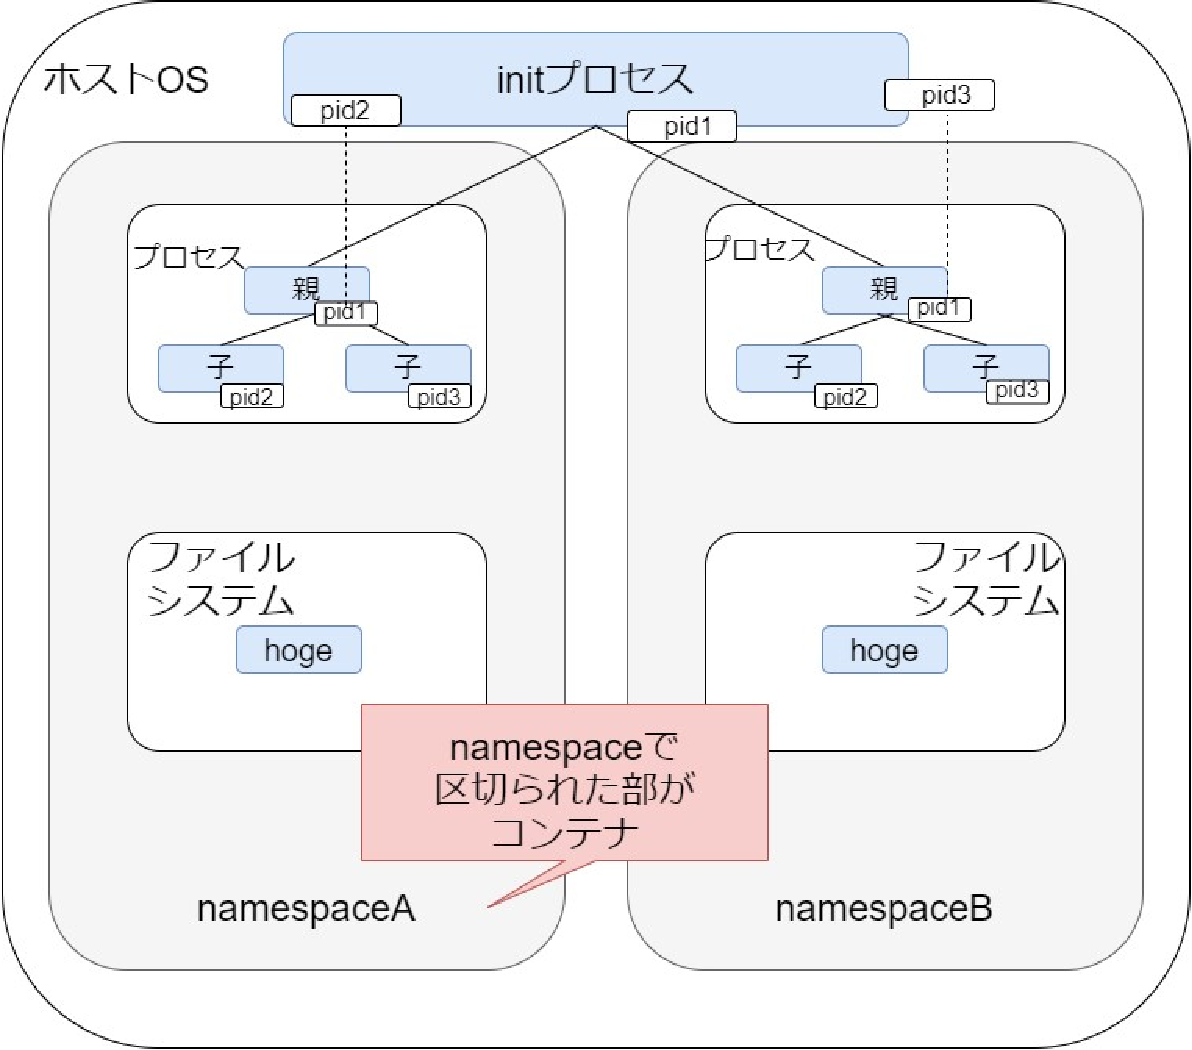
\includegraphics[width=13cm,height=12cm,keepaspectratio]{namespace-crop.pdf}\\
        %includegraphicsの詳しい使い方ははLaTeXの参考書を参照.
    \end{center}
    \caption{コンテナの構成図}
    \label{namespace}
\end{figure}

ホストOS上にnamespaceAとnamespaceBを作成し,それぞれのnamespaceの空間で全く独立したファイル構造やプロセス空間を持つことができる.
このように分離された環境をコンテナという.
コンテナのプロセス空間に関しては,実際にはホストOS上で動作しているプロセスIDとコンテナ上で動作しているプロセスIDをマッピングしているテーブルが存在する.
これを用いてホストOS上ではpid2として認識されているが,コンテナ上ではpid1として認識されていることになる.

このことによりnamespaceを利用すると,プロセス空間やファイルシステムを一つのOSの中で分離できるので,namespaceで区切られた部分であるコンテナは全く異なるOSのようにふるまうことが可能となる.

\subsubsection{Docker Engine}
\ref{sec:container}節で述べたようにDockerはコンテナを用いて動作している.
しかし,プロセスをコンテナ上で稼働させるためには,OSの動作に必要なコマンドやライブラリが必要になる.
これを実現するためには相当量のコマンドを発行しなければならない.
そこでDockerは,Docker Engineを作成した.
Docker Engineは主に以下のコンポーネントからなるクライアントサーバ型アプリケーションである.

\begin{description}
    \item[・サーバ]\mbox{}\\
        長時間稼働する種類のプログラムでありデーモン・プロセスと呼ばれる.
    \item[・REST API]\mbox{}\\
        プログラムとデーモンとの間での通信方法を定義し,何をなすべきかを指示する.
    \item[・コマンドライン・インターフェイス(CLI)]\mbox{}\\
        クライアント.dockerコマンドなど.
\end{description}

デーモンは,Dockerオブジェクトを作成,管理する.
Dockerオブジェクトとは,イメージ,コンテナ,ネットワーク,データ,ボリュームなどを表す.

CLIはDocker REST APIを通じて,スクリプトのコマンド実行により,Dockerデーモンを制御,入出力を実行する.
Dockerアプリケーションの多くが,基本的なところでこのAPIやCLIを利用している.

また,Dockerの内部には以下の3つのコンポーネントが存在する.

\begin{itemize}
    \item Dockerイメージ
    \item Dockerレジストリ
    \item Dockerコンテナ
\end{itemize}

Dockerイメージとは,読み込み専用なテンプレートである.
DockerイメージはDockerコンテナ作成時に使用される.
各イメージはレイヤの積み重ねで構成される.
また,新しいイメージの構築や既存のイメージの更新だけでなく,他人が作成したDockerイメージをダウンロードして使用することも可能である.
DockerはUnionFS\cite{Unionfs}を用いて各イメージのレイヤを単一のイメージに連結する.
これにより,Dockerイメージに変更を加えた場合,変更したい部分のレイヤを追加もしくは更新するだけでよいため,構築に時間がかからず早く簡単にイメージを提供できる.

Dockerレジストリとは,イメージを保持するものである.
パブリックもしくはプライベートに保管されているイメージのアップデートやダウンロードを実行することができる.
パブリックなDockerレジストリとしてDocker Hub\cite{dockerhub}が提供されている.

Dockerコンテナとは,ディレクトリと似たようなもので,アプリケーションの実行に必要なすべてが含まれている.
各コンテナはDockerイメージによって作成される.
Dockerコンテナは実行・開始・停止・移動・削除できる.
各コンテナは隔離されているため,安全なアプリケーションのプラットフォームとして動作する.


\subsubsection{Docker Compose}
Composeとは,複数のコンテナを定義し実行するDockerアプリケーションの為のツールである.
ComposeにおいてはYAML\cite{YAML}ファイルを使ってアプリケーションサービスの設定する.
コマンド一つ実行するだけで,設定内容に基づいたアプリケーションを生成,起動する.

Composeを使うには基本的に3つのステップを踏む.

\begin{enumerate}
    \item アプリケーション環境をDockerfileに定義する.
    \item アプリケーションを構成するサービスをdocker-compose.ymlファイル内に定義する.
    \item docker-compose upを実行したら,Composeはアプリケーション全体を起動・実行する.
\end{enumerate}

\newpage
\subsubsection{コマンド一覧}
DockerとDocker Composeで使用する代表的なコマンド一覧とコマンドの説明を表\ref{docker_command}に示す.


\begin{table}[htb]
    \begin{center}
        \caption{Dockerコマンド一覧}
        \begin{tabularx}{\textwidth}{|l|X|}\hline
            docker run -it [イメージ名] /bin/bash & dockerコンテナを起動し,ログイン \\ \hline
            docker run -p [外部ポート]:[コンテナポート] & コンテナに外部からアクセスする \\ \hline
            docker run -v [ホストボリュームパス]:[コンテナ内パス] [コンテナイメージ名] & コンテナのボリュームをホストにマウントする \\ \hline
            docker save [イメージ名] \textgreater [ファイル名].tar.gz & dockerイメージをtar.gz形式で保存する\\ \hline
            docker load \textless [ファイル名].tar.gz & tar.gz形式のdockerイメージを取り込む \\ \hline
            docker exec -it [コンテナID/コンテナ名] /bin/bash & 起動中のコンテナにログイン \\ \hline
            docker cp [ホストファイルパス] [コンテナID]:[コンテナコピー先パス] & 起動中コンテナにホストからファイルをコピー \\ \hline
            docker commit [起動中のコンテナID] [イメージ名] & 起動中のコンテナをイメージとして保存 \\ \hline
            docker start [コンテナ名] & コンテナの開始 \\ \hline
            docker stop [コンテナ名] & コンテナの停止 \\ \hline
            docker restart [コンテナ名] & コンテナの再起動 \\ \hline
        \end{tabularx}
        \label{docker_command}
    \end{center}
\end{table}


\begin{table}[htb]
    \begin{center}
        \caption{Docker Composeコマンド一覧}
        \begin{tabularx}{\textwidth}{|l|X|}\hline
            docker-compose ps & コンテナの一覧を表示 \\ \hline
            docker-compose images & イメージの一覧を表示 \\ \hline
            docker-compose up --build & コンテナのビルドと起動 \\ \hline
            docker-compose down & docker-compose.ymlで起動したコンテナの削除 \\ \hline
            docker-compose start & docker-compose.ymlでビルドしたコンテナの起動 \\ \hline
            docker-compse stop [サービス名] & docker-compose.ymlで起動しているコンテナの停止 \\ \hline
            docker-compse exec [サービス名] [コマンド] & docker-compose.ymlで起動したコンテナにログインしてコマンドを発行 \\ \hline 
        \end{tabularx}
        \label{docker-compose_command}
    \end{center}
\end{table}





\subsection{Python}
\subsubsection{概要}
Python\cite{python}はWindows,Linux/Unix,Mac OS X などの主要なオペレーティングシステムおよびJavaや.NETなどの仮想環境でも動作するインタプリタ形式の,対話的な,オブジェクト指向プログラミング言語である.
この言語には,モジュール,例外,動的な型付け,超高水準の動的データ型,およびクラスが取り入れられている.
Pythonはオブジェクト指向プログラミングを超えて,手続き型プログラミングや関数型プログラミングなど複数のプログラミングパラダイムをサポートしている.
また,多くのシステムコールやライブラリだけでなく,様々なウィンドウシステムへのインターフェースがあり,C\cite{Clang}やC++\cite{cplusplus}で拡張することもできる.

\subsubsection{Django}
Django\cite{Django}は,Pythonで実装されたオープンソースのWebアプリケーションフレームワークの一つである.
Djangoが作られた時の目的として,複雑なデータベース主体のウェブサイトを簡単に構築するというものがある.
これを実現するため,Djangoではコンポーネントの再利用性,素早い開発の原則に力を入れている.
Djangoには以下のような特徴がある.

\begin{description}
    \item[・高速な動作]\mbox{}\\
        Djangoには標準で分散型のキャッシュシステムであるmemcached\cite{memcached}が備え付けられており,キャッシュ機能が強力である.
    \item[・フルスタック・フレームワーク]\mbox{}\\
        Djangoには,Webアプリケーションの実装に必要な,ユーザ認証,管理画面,RSSフィードなどの機能があらかじめ含まれている.
    \item[・セキュリティ的に安全な設計]\mbox{}\\
        Djangoでは,デフォルトでパスワードなどはハッシュ化しデータベースに格納する.
        また,SQLインジェクション,クロスサイトスクリプティング,クロスサイトリクエストフォージェリなどの多くの脆弱性についても保護を有効にしている.
    \item[・自由に選択できるプラットフォーム]\mbox{}\\
        Djangoは,そのすべてがPythonから作成されている.これにより,PythonがLinux,Windows,MacOS Xなどで実行できるようにDjangoも多くのプラットフォームで動作可能である.
\end{description}

\newpage
また,Djangoの機能構成としてMVT(Model・View・Template)というものがある.
DjangoはMVTのもと,ルーティングというリクエストを振り分ける機能を用いてアプリケーションを動作させている.
Djangoがどのように動作するかを図\ref{django_work}に示す.

\begin{figure}[htbp]
    \begin{center}
        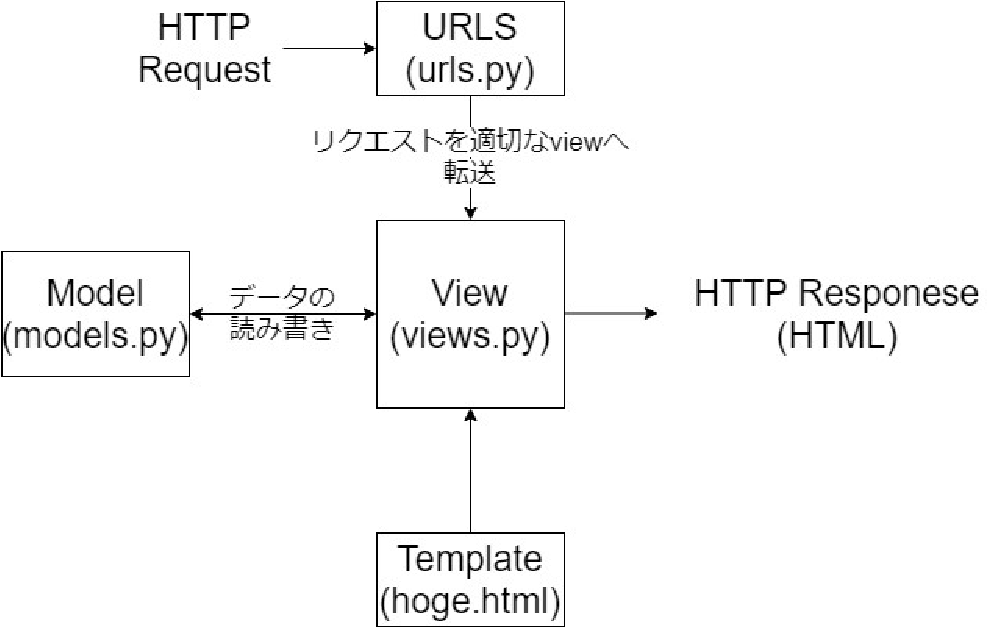
\includegraphics[width=13cm,height=12cm,keepaspectratio]{django_work-crop.pdf}\\
        %includegraphicsの詳しい使い方ははLaTeXの参考書を参照.
    \end{center}
    \caption{Djangoの動作の概要図}
    \label{django_work}
\end{figure}

URLSは単一URLから単一の関数を介してすべてのリクエストを処理することは可能だが,各リソースを処理する別々のView関数を作成する方がメンテナンスが容易なため,URLをマッピングしている.
これにより,URLに含まれる特定のパターンの文字列もしくは数字を照合し,これらをデータとしてView関数に渡して処理を行っている.

Viewは,HTTPリクエストを受け取り,HTTPレスポンスを返す関数である.
Viewはモデルを介して要求を満たすために必要なデータにアクセスし,レスポンスのフォーマットをTemplateに委任する.

Modelは,アプリケーションのデータ構造を定義し,データベース内のレコードを追加,変更,削除,および照会するための機能を提供するPythonオブジェクトである.

Templateは,ファイル構造やレイアウトを定義するテキストファイルで,プレースホルダを使用して実際のコンテンツを表示する.
Viewは,モデルから取得したデータとHTMLテンプレートを使用して動的にHTMLページを作成できる.
また,Templateを利用して,HTMLだけではなく,あらゆる種類のファイルの構造を定義できる.

\newpage
続いて,Djangoは複雑なデータベース主体のウェブサイトを簡単に構築するため,データベースを操作する3つの機能がある.
\begin{description}
    \item[・Djangoシェル]\mbox{}\\
        Djangoアプリケーションの環境を有効にしたままコマンドで操作が可能.
    \item[・マイグレーション]\mbox{}\\
        データベースの操作を一括に実行・取り消すことが可能.
    \item[・管理サイト]\mbox{}\\
        Webブラウザで,データベースを操作することが可能. 
\end{description}
これらの機能を用いることにより,複雑なデータベース主体のウェブサイトを簡単に構築できる.

最後にDjangoで主に使用するコマンド一覧とその説明を表\ref{django_command}に示す.

\begin{table}[htb]
    \begin{center}
        \caption{Dockerコマンド一覧}
        \begin{tabularx}{\textwidth}{|l|X|}\hline
            manage.py createsuperuser & 管理者ユーザを作成. \\ \hline
            manage.py changepassword & ユーザのパスワードを変更. \\ \hline
            manage.py check & プロジェクトの構成チェック. \\ \hline
            manage.py dbshell & データベース管理用のシェルを起動. \\ \hline
            manage.py dumpdata & データベースの内容をJson等の形式でエクスポート. \\ \hline
            manage.py loaddata & データベースにdumpファイルをインポート. \\ \hline
            manage.py makemigrations & マイグレーションファイルの作成. \\ \hline
            manage.py migrate & データベースにマイグレーションを適用. \\ \hline
            manage.py shell & 管理者用のコマンドシェルを起動し対話モードに入る. \\ \hline
            manage.py startapp & 新規アプリケーションの作成. \\ \hline
            manage.py startproject & プロジェクトディレクトリの作成. \\ \hline
            manage.py test & テストフレームワークの実行. \\ \hline
            manage.py testserver & 検証用サーバを起動. \\ \hline
            manage.py collectstatic & staticファイルの収集. \\ \hline
            manage.py runserver & アプリケーションの起動. \\ \hline
        \end{tabularx}
        \label{django_command}
    \end{center}
\end{table}

\subsubsection{Django REST framework}
Django REST framework\cite{drf}とはDjangoを使ってRESTfulなAPIを開発するために利用されるライブラリである.
Django REST frameworkを動作させるには,以下の要件を満たさなければならない.
\begin{enumerate}
    \item Python (3.5,3.6,3.7,3.8,3.9)
    \item Django (2.2,3.0,3.1)
\end{enumerate}




\subsection{その他関連技術}
\subsubsection{Go}
Go\cite{golang}は静的型付けの効率と安全性,動的型付けのプログラミングの容易さを兼ね備えたプログラミング言語である.
また,Goのコンパイラ,ツール,およびソースコードはすべてフリーなオープンソースである.


\subsubsection{PostgreSQL}
PostgreSQL\cite{postgres}とは,Linux,Windows,MacOS Xに対応した,オープンソースのリレーショナルデータベース管理システム(RDBMS)である.
特徴として以下のようなものがある.
\begin{description}
    \item[拡張性]\mbox{}\\
        PostgreSQLでは,アーキテクチャが拡張可能である.このことにより,データベース内の手順のカスタマイズや自動化に使用できるユーザ定義関数とサードパーティライブラリへのサポートが可能となる.
    \item[同時実行性]\mbox{}\\
        PostgreSQLでは,マルチバージョン同時実行制御があり,ユーザは同じデータベースの書き込みと読み取りが可能となっている.
    \item[標準SQLへの準拠]\mbox{}\\
        PostgreSQLでは,ISO/IECの標準SQLにならった実装となっている.
\end{description}


\subsubsection{Chart.js}
Chart.js\cite{chartjs}とは,HTML5のCanvasを使用したグラフ描画ライブラリである.
Chart.jsはオープンソースなプロジェクトで,8つのチャートタイプと優れたレスポンシブを有している.
8つのチャートタイプは以下の通りである.
\begin{itemize}
    \item 線グラフ
    \item 棒グラフ
    \item レーダーチャート
    \item 円グラフ
    \item 鶏頭図
    \item バブルチャート
    \item 散布図
    \item エリアチャート
\end{itemize}
また,2種類以上のチャートを複合した複合グラフも作成できる.


\subsubsection{Json}
Json\cite{json}(Javascript Object Notation)は,軽量なデータ交換フォーマットである.
人間にとって読み書きが容易で,マシンにとってもパースや生成を行える.

\subsubsection{NGINX}
NGINX\cite{nginx}は,フリーでオープンソースなWebサーバである.
HTTP,HTTPS,SMTP,POP3,IMAPのリバースプロキシ機能や,ロードバランサ,HTTPキャッシュなどの機能を持つ.

\subsubsection{Gunicorn}
Gunicorn\cite{gunicorn}は,UNIXのためのPython WSGI HTTP Serverである.
WSGI\cite{wsgi}とは,PythonにおいてWebサーバとWebアプリケーションを接続するための,標準化されたインターフェース定義のことである.


%
% 研究内容
%
\section{研究内容}\label{se3}
本章では,概要,開発環境,関連研究,システム概要を述べた後に,開発した本プラットフォームの詳細について述べる.

\subsection{概要}
本研究の目的は,情報倫理教育に関する学習を支援することである.そのため,学習者が情報倫理に関して学ぶとき,手軽に学習する環境を構築する必要がある.これを解決するために本研究では学習をインターネット上で手軽に学習するためにwebアプリケーションを用いたeラーニングプラットフォームを開発した.
本プラットフォームは,情報倫理に関して学習する学習者と情報倫理に関するコンテンツを提供する教材提供者を対象としたシステムである.教材提供者に対して本プラットフォームではコンテンツ提供機能,統計情報提供機能,コンテナ管理機能を用意している.
教材提供者はこれらの機能を用いることにより情報倫理に関するコンテンツをwebアプリケーション上に投稿でき,学習者はそれらのコンテンツを用いて情報倫理に関する学習を行える.

\subsection{開発環境}
本プラットフォームを作成するにあたって使用したPCのスペックと開発環境を表\ref{env}に示す.

\begin{table}[htb]
    \begin{center}
        \caption{PCのスペックと開発環境}
        \begin{tabular}{|l|l|} \hline
            CPU & Intel Core i7 @ 3.70GHz \\ \hline
            Memory &  24.0GB \\ \hline
            OS & Windows 10 Education 64-bit \\ \hline
            開発環境 & 
            \begin{tabular}{l}
            Docker version 20.10.0, build 7287ab3 \\ docker-compose version 1.27.4, build 40524192
            \end{tabular}\\ \hline
        \end{tabular}
        \label{env}
    \end{center}
\end{table}

\subsubsection{クライアントシステムとサーバシステムの開発環境}
クライアントシステムとサーバシステムの開発にはDockerのコンテナを用いた.表\ref{client},表\ref{server}にそれぞれの開発環境を示す.

\begin{table}[htb]
    \begin{center}
        \caption{クライアントシステムの開発環境}
        \begin{tabular}{|l|l|} \hline
            OS & Alpine Linux(3.12.3) \\ \hline
            使用言語・フレームワーク & 
            \begin{tabular}{l}
            Python 3.7.9 \\ Django 3.0.2 \\
            \end{tabular}\\ \hline
        \end{tabular}
        \label{client}
    \end{center}
\end{table}

\begin{table}[htb]
    \begin{center}
        \caption{サーバシステムの開発環境}
        \begin{tabular}{|l|l|} \hline
            OS &  Debian GNU/Linux 10 (buster) \\ \hline
            使用言語・フレームワーク & 
            \begin{tabular}{l}
            go version go1.15.6 linux/amd64 \\ djangorestframework 3.12.1 \\ 
            \end{tabular}\\ \hline
        \end{tabular}
        \label{server}
    \end{center}
\end{table}
\newpage
\subsection{関連研究}
関連研究として,上田氏らの「倫倫姫プロジェクト-学人連携Moodleによる多言語情報倫理eラーニング-」\cite{rinri}がある.

倫倫姫プロジェクトでは大学の情報倫理教育における以下3つの問題を解決している.

\begin{enumerate}[(i)]
    \item 標準化と可視化がなされていない \label{i}
    \item 留学生への教育が困難 \label{ii}
    \item 持続可能性が低い \label{iii}
\end{enumerate}

(\ref{i})を解決するために,倫倫姫ではサンプル規程集「A3301 教育テキスト作成ガイドライン(一般利用者向け)」に準拠することで,内容を標準化した.
また,受講履歴を閲覧でき受講者の学習状況の可視化も実現した.

(\ref{ii})を解決するために,倫倫姫では英語,中国語,韓国版を作成しており,各言語圏の文化の違いも考慮しコンテンツを作成することで解決した.

(\ref{iii})を解決するために,倫倫姫ではSCORMが規定するeラーニングコンテンツパッケージを利用した.
これは,パッケージ構造とリソースを記述するマニフェストファイル(imsmanifest.xml)とそれから参照される物理ファイル(HTML,swfなど)をファイル単位で修正可能なため継続的な改訂を可能としている.

本研究でも(\ref{i}),(\ref{iii})については同様に本プラットフォームで解決している.
(\ref{i})に関しては,コンテンツ提供機能により,教材提供者間でコンテンツを共有できることから解決している.
(\ref{iii})に関しては,本プラットフォームではコンテンツはWebアプリケーション上で管理しており,コンテンツの修正もWeb上から行えることから解決している.

一方,本プラットフォームにおいては,コンテンツに関してはマークダウン形式で記入可能なことから,過去のコンテンツを本プラットフォーム上に移行することが簡単である.
また,コンテナ管理機能により,過去に作成したアプリケーションに関しても本プラットフォーム上に移行することが簡単である.



\newpage
\subsection{システム概要}
\subsubsection{要件定義}
本システムはサーバ,クライアントで以下の要件を満たす必要がある.

まずサーバの要件を示す.

\begin{itemize}
    \item Dockerの動作: すべての開発にDockerを用いる
    \item Webサーバの動作: Webアプリケーションの公開に用いる
    \item Pythonの動作: Djangoの動作に用いる
    \item Goの動作: APIの動作に用いる
    \item PostgreSQLの動作: ユーザの管理等のデータベースとして用いる
\end{itemize}

サーバはWebサーバを用いてクライアントをネットワークに公開し,Dockerを用いてPythonとGoとPostgreSQLを動作させる.
PythonはDjangoを動作させ,クライアントにGUI等を提供する.
GoはAPI作成に用いて,Dockerを操作する.
PostgreSQLは,Djangoを通してクライアントから入力されたデータ等を保存する.

続いて,クライアントの要件を示す.

\begin{itemize}
    \item html5が解釈できるWebブラウザの動作: クライアントの動作環境となる 
\end{itemize}

クライアントはWebアプリケーションであり,html5を解釈できるWebブラウザ上で動作する.
クライアントは教材提供者と学習者に対してGUIを提供する.
詳細は,\ref{sec:fun1}節,\ref{sec:fun2}節,\ref{sec:fun3}節で述べる.

また,作成する機能は以下の要件を満たすように作成した.

\begin{itemize}
    \item 日々変化する情報倫理に対応する為の機能を作成する
    \item 年代,性別の違いによる情報倫理に関する意識の違いを確認する為の機能を作成する
    \item 本アプリケーション以外のアプリケーションを本アプリケーションでも利用可能にする機能を作成する
\end{itemize}

日々変化する情報倫理に対応する為の機能は,コンテンツ提供機能として作成し,これを用いてコンテンツを素早く投稿,編集する.
年代,性別の違いによる情報倫理に関する意識の違いを確認する為の機能は,統計情報提供機能として作成し,年代や性別をグラフとして提示する.
本アプリケーション以外のアプリケーションを本アプリケーションでも利用可能にする機能は,コンテナ管理機能として作成し,Dockerを用いたアプリケーションを本プラットフォーム上でも利用可能にする.

\newpage
\subsubsection{システム構成}
本システムの構成を図\ref{system}に示す.本システムはDjangoで構成されるアプリケーション部(以下,クライアント),およびGoとdjangorestframeworkで構成されるサーバ部(以下,サーバ)から構築される.
サーバはAPIを用いて統計情報提供機能とコンテナ管理機能を動作させる.

\begin{figure}[htbp]
    \begin{center}
        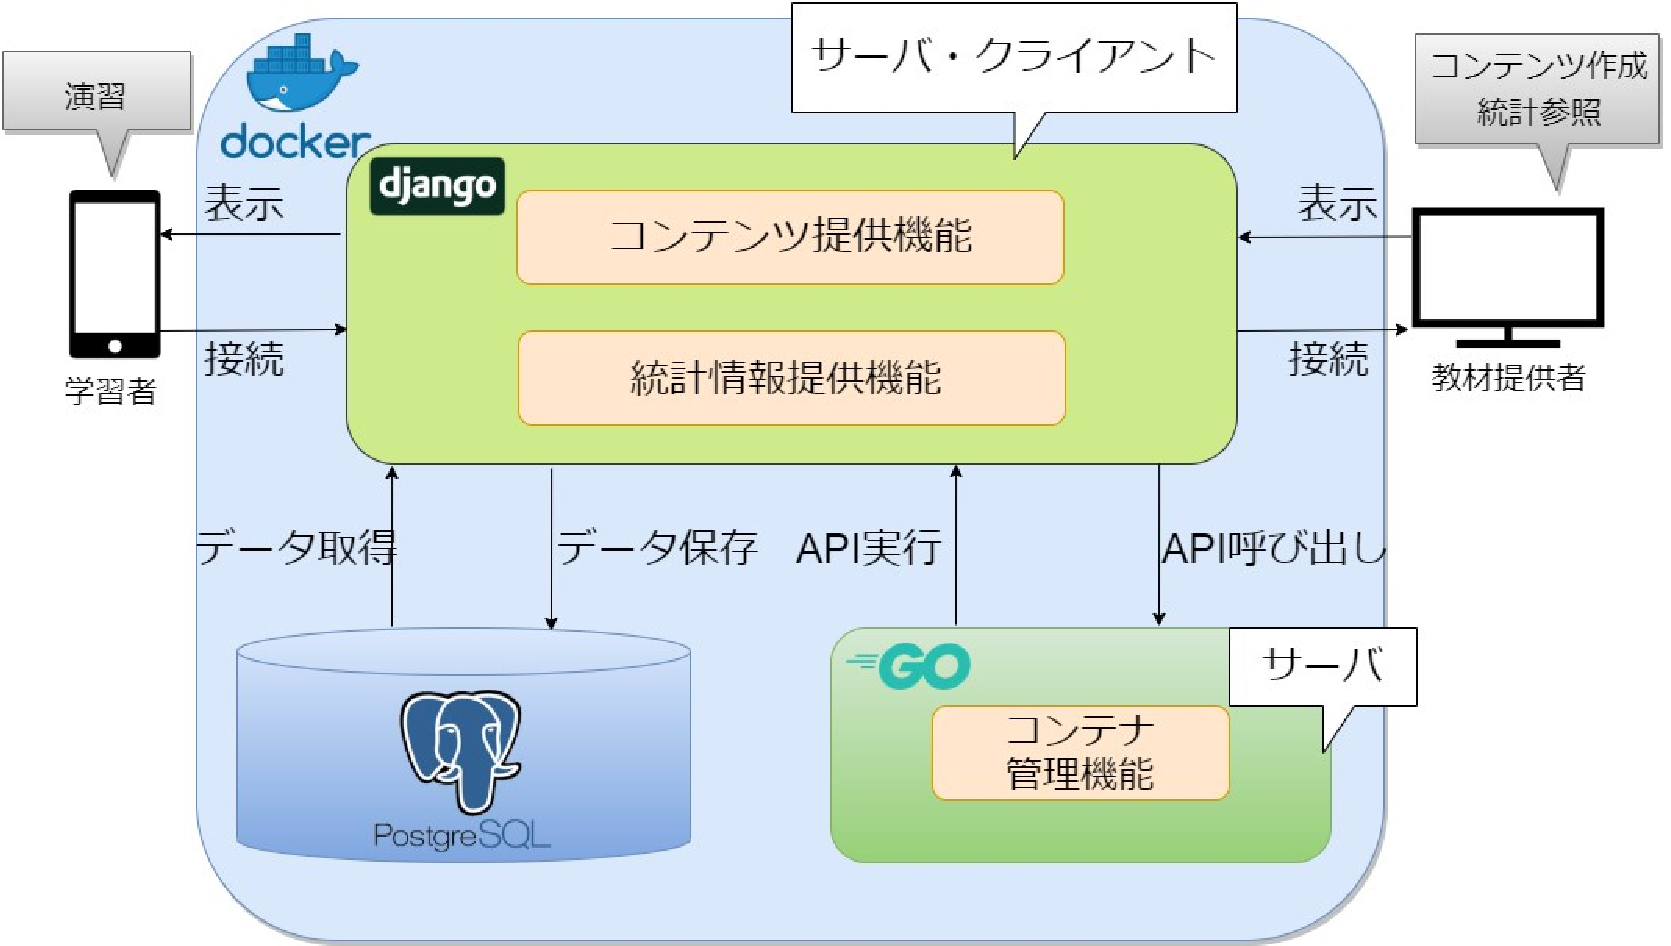
\includegraphics[width=16cm,height=15cm,keepaspectratio]{system-crop.pdf}\\
        %includegraphicsの詳しい使い方ははLaTeXの参考書を参照.
    \end{center}
    \caption{システム構成}
    \label{system}
\end{figure}


コンテンツ提供機能のGUIを図\ref{teikyou}に,統計情報提供機能のGUIを図\ref{toukei}に,コンテナ管理機能のGUIを図\ref{kanri}にそれぞれ示す.

\newpage
教材提供者は図\ref{teikyou}のコンテンツ提供機能を用いて情報倫理に関するコンテンツを提供する.

\begin{figure}[htbp]
    \begin{center}
        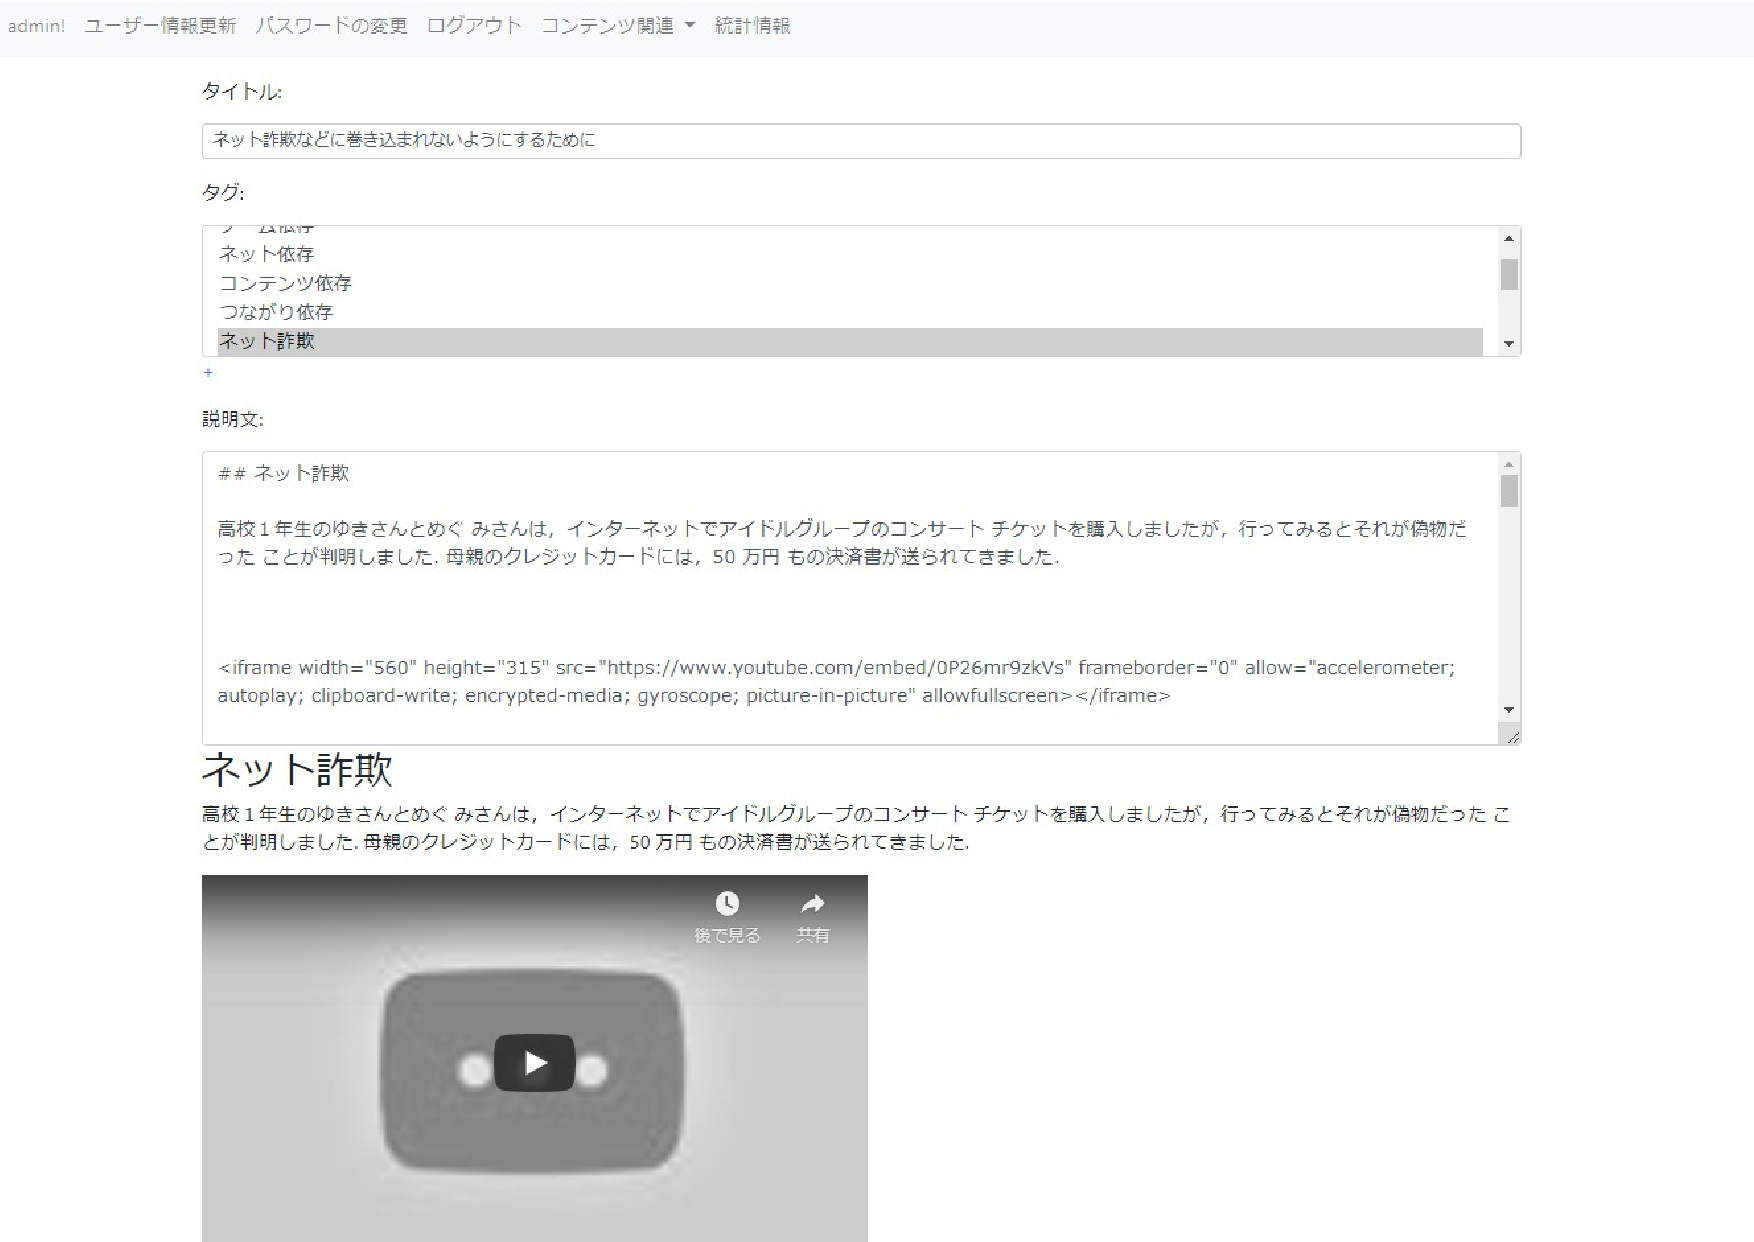
\includegraphics[width=18cm,height=17cm,keepaspectratio]{create_content-crop.pdf}\\
        %includegraphicsの詳しい使い方ははLaTeXの参考書を参照.
    \end{center}
    \caption{コンテンツ提供機能のGUI}
    \label{teikyou}
\end{figure}

\newpage
図\ref{toukei}の統計情報提供機能では,教材提供者が学習者の回答情報等をグラフとして確認できる.
\begin{figure}[htbp]
    \begin{center}
        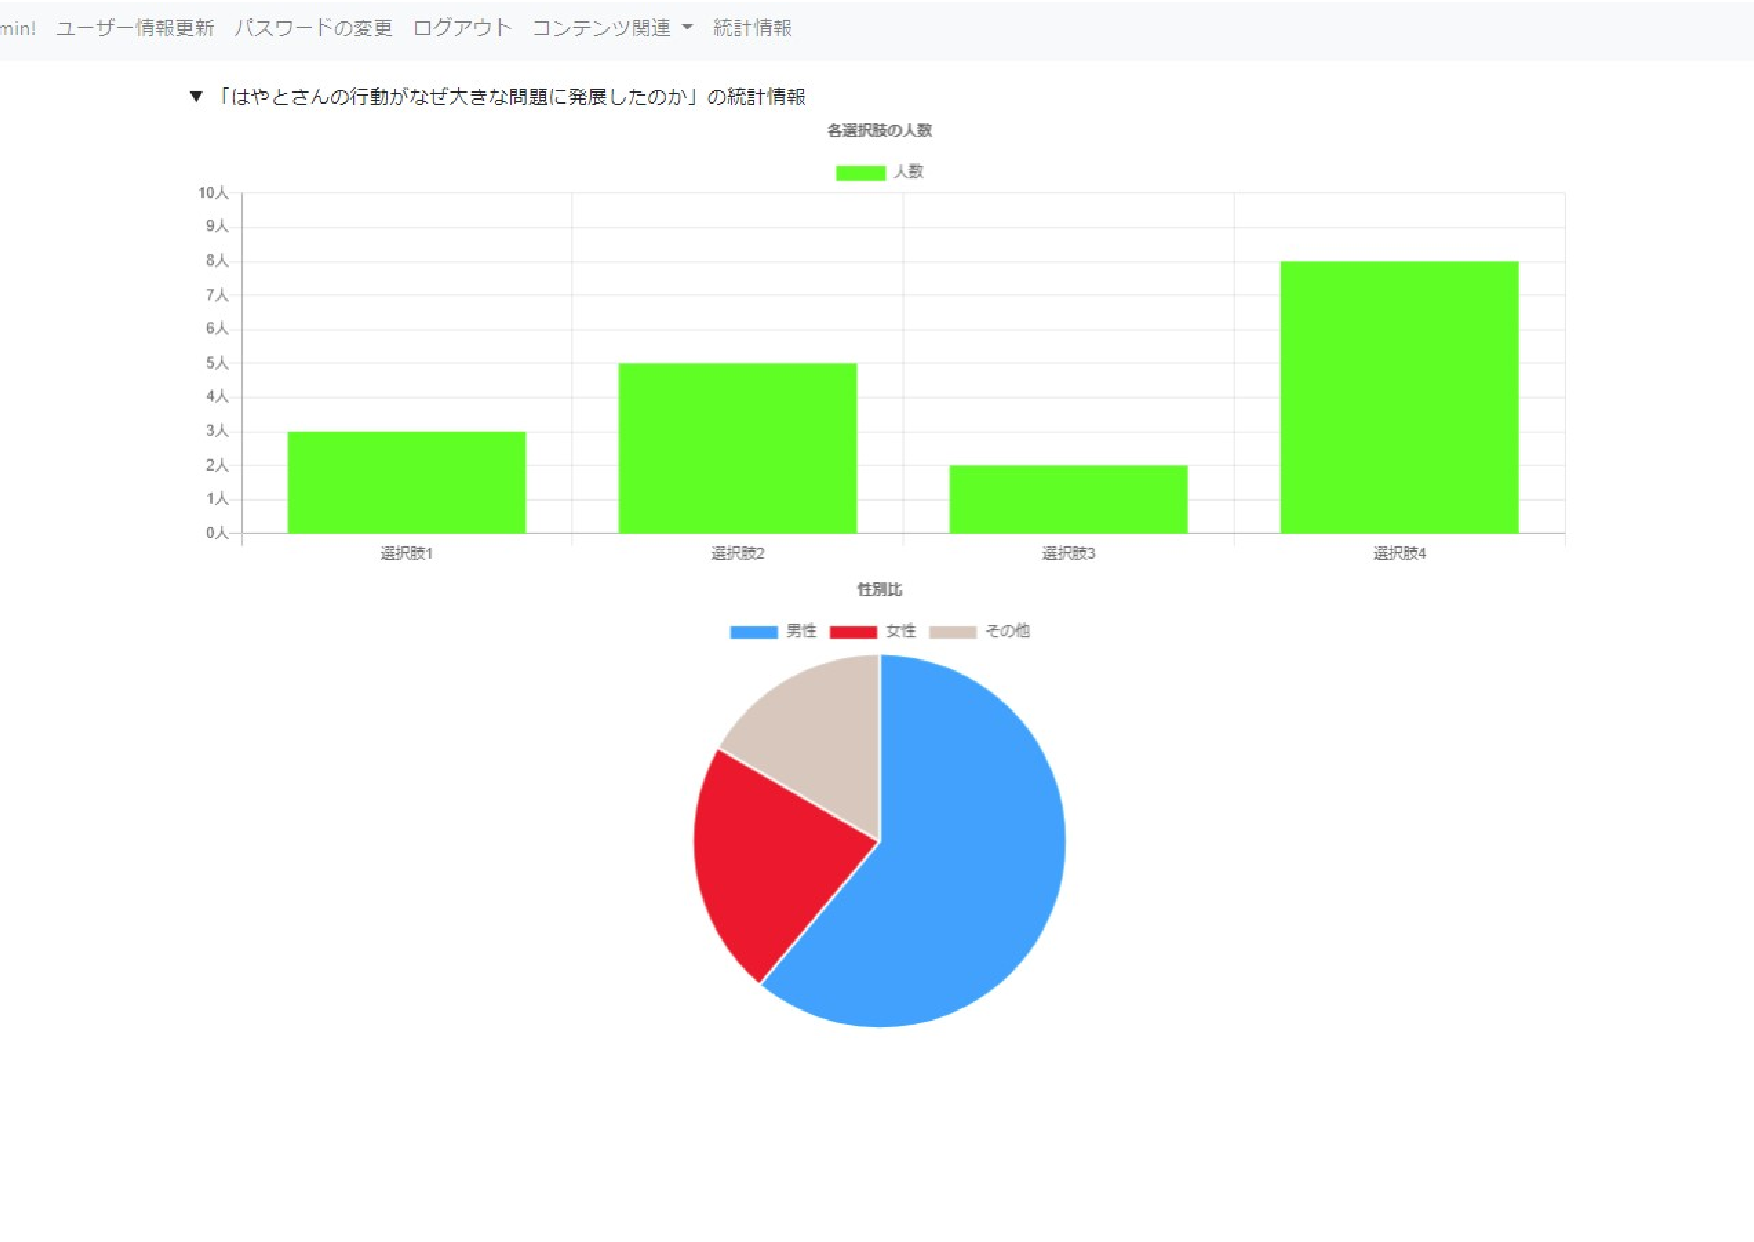
\includegraphics[width=16cm,height=15cm,keepaspectratio]{toukei-crop.pdf}\\
        %includegraphicsの詳しい使い方ははLaTeXの参考書を参照.
    \end{center}
    \caption{統計情報提供機能のGUI}
    \label{toukei}
\end{figure}

\newpage
図\ref{kanri}のコンテナ管理機能では教材提供者がDockerを用いて作成した他の教育アプリケーションを本プラットフォームでも利用することが可能となる.
\begin{figure}[htbp]
    \begin{center}
        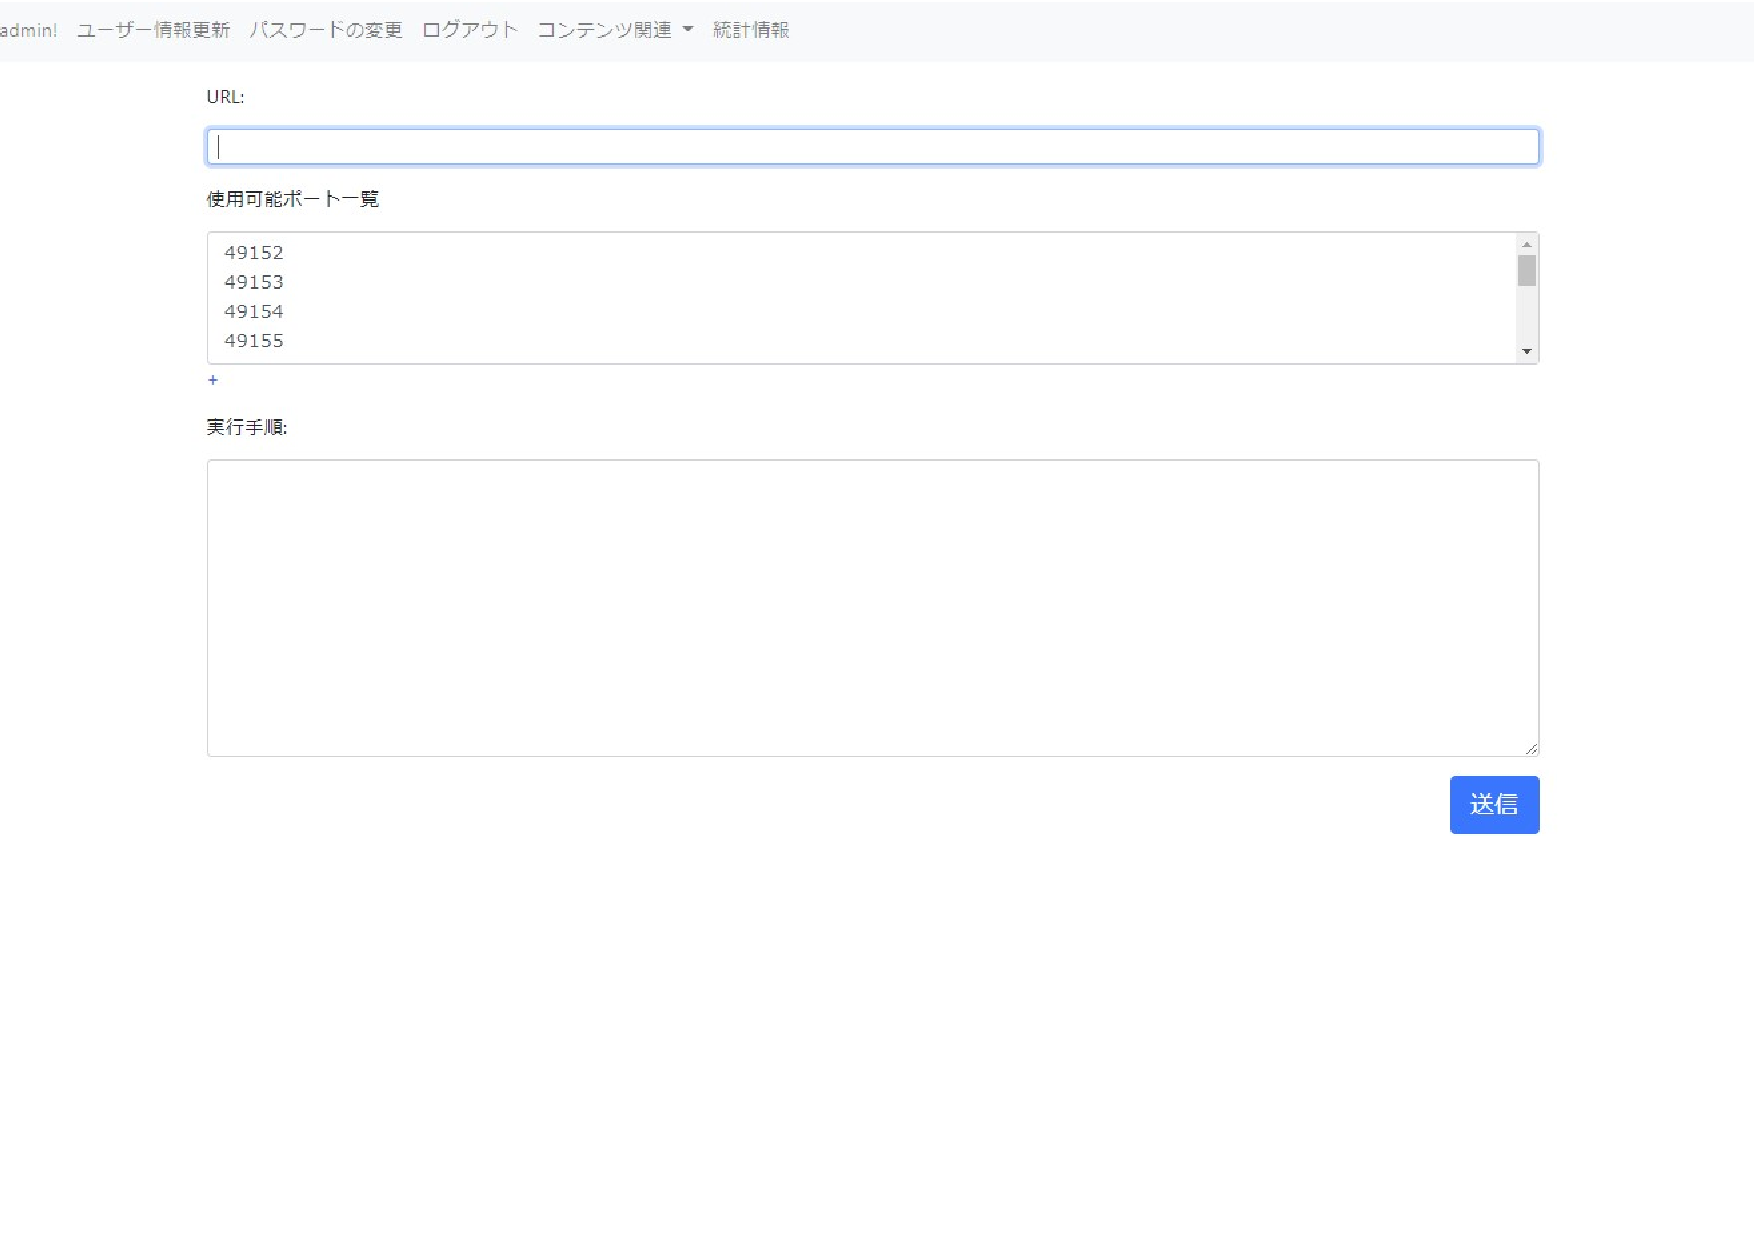
\includegraphics[width=18cm,height=17cm,keepaspectratio]{container_management-crop.pdf}\\
        %includegraphicsの詳しい使い方ははLaTeXの参考書を参照.
    \end{center}
    \caption{コンテナ管理機能のGUI}
    \label{kanri}
\end{figure}

\newpage
学習者は図\ref{teikyou}のコンテンツ提供機能を用いて作成されたコンテンツを図\ref{naiyou}のようにして閲覧,学習することが可能である.
\begin{figure}[htbp]
    \begin{center}
        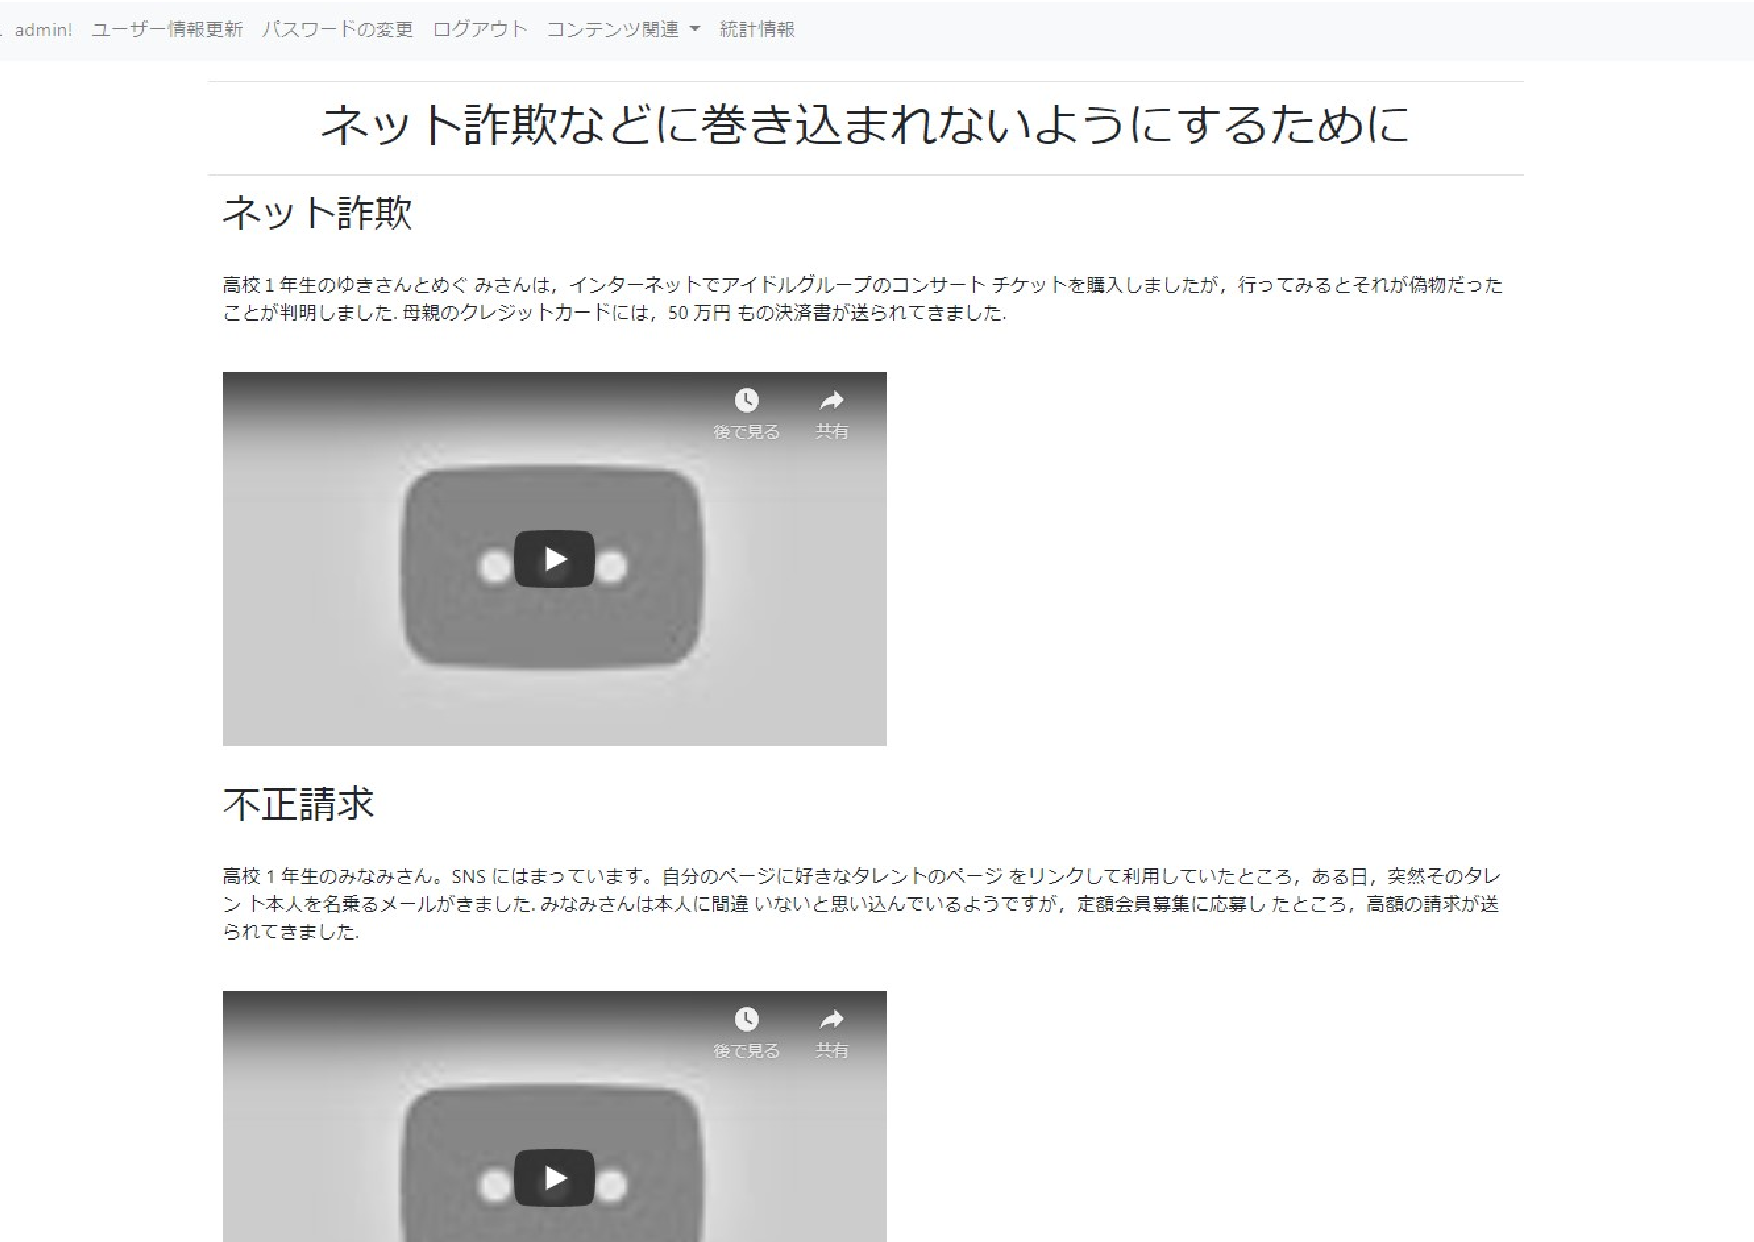
\includegraphics[width=18cm,height=17cm,keepaspectratio]{naiyou-crop.pdf}\\
        %includegraphicsの詳しい使い方ははLaTeXの参考書を参照.
    \end{center}
    \caption{コンテンツ閲覧時のGUI}
    \label{naiyou}
\end{figure}

\newpage
\subsubsection{システムの内部構成}
クライアントの内部構成を図\ref{client_naibu}に示す.はじめに,教材提供者および学習者が各々ネットワークに接続できる環境を用意し,Webブラウザを立ち上げ,特定のIPアドレスを入力しログインする.
ただし,教材提供者が本プラットフォームの機能を利用するにはログインは必須であるが,学習者は必須ではない.

Webブラウザで本プラットフォームに接続しログインした後,教材提供者はGUIのコンテンツ提供機能,統計情報提供機能,コンテナ管理機能を使用できる.
コンテンツ提供機能は教材提供者が入力した内容をサーバを介しデータベースに保存する.
統計情報提供機能はデータベースからサーバを介しデータを取得しWebブラウザ上に情報を表示する.
コンテナ管理機能は教材提供者が入力した内容をGoで作成したAPIで実行し,Dockerのコマンドを用いてコンテナが建ち上がっていることを確認し,建ち上がっていた場合それにアクセスするURLを画面上に発行する.

\begin{figure}[htbp]
    \begin{center}
        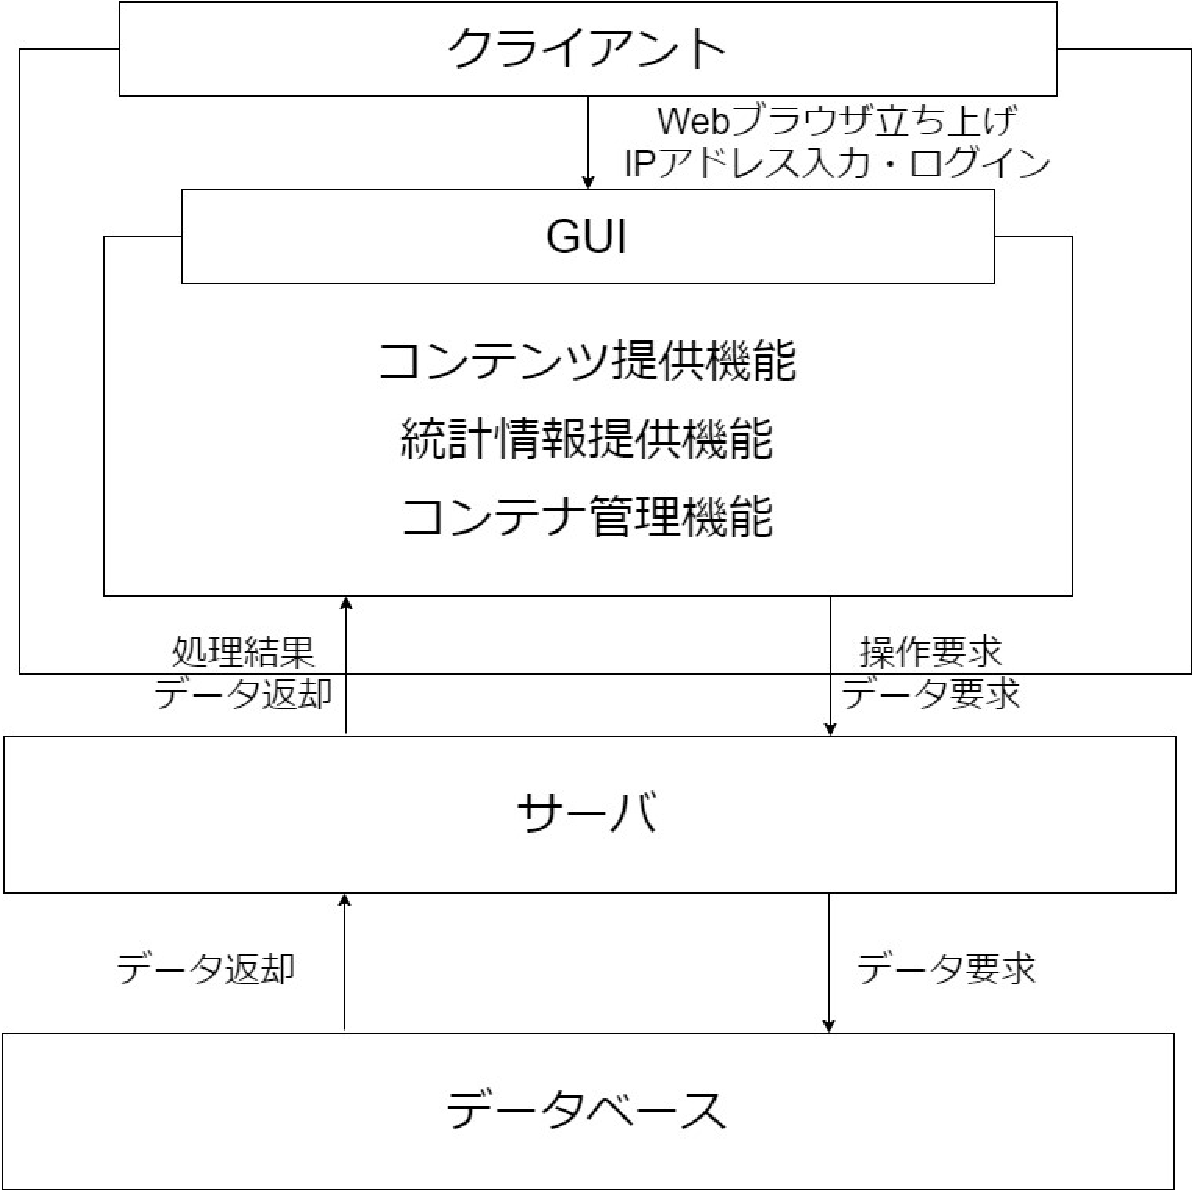
\includegraphics[width=13cm,height=12cm,keepaspectratio]{client_arch-crop.pdf}\\
        %includegraphicsの詳しい使い方ははLaTeXの参考書を参照.
    \end{center}
    \caption{クライアントの内部構成}
    \label{client_naibu}
\end{figure}

\newpage
続いて,サーバの内部構成を図\ref{server_naibu}に示す.サーバはDjangoを用いて作成されたDjango処理部とGoを用いて作成されたGo処理部,データを保存するためのデータベース処理部がある.
サーバはクライアントからの通信が行われた場合に動作する.それぞれの処理部の内容について以下に示す.

\begin{figure}[htbp]
    \begin{center}
        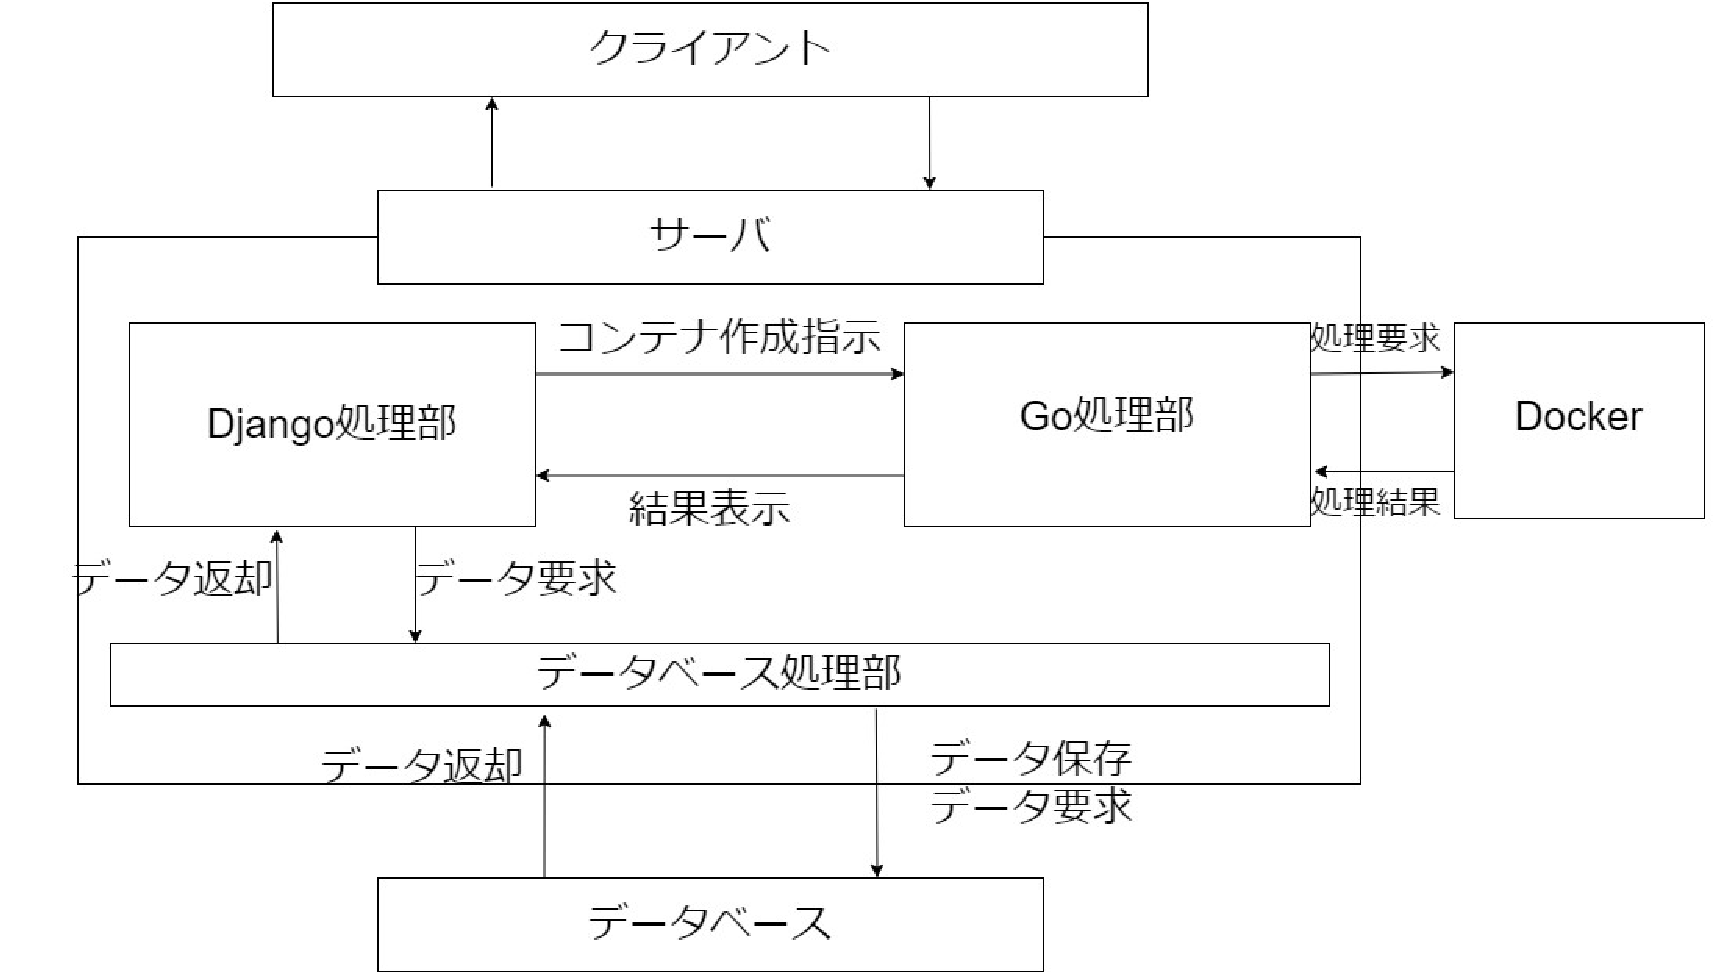
\includegraphics[width=17cm,height=16cm,keepaspectratio]{server_arch-crop.pdf}\\
        %includegraphicsの詳しい使い方ははLaTeXの参考書を参照.
    \end{center}
    \caption{サーバの内部構成}
    \label{server_naibu}
\end{figure}

\begin{description}
    \item[・Django処理部]\mbox{}\\
        Django処理部では,クライアントからフォームに従って入力されたデータをデータベースに登録,抽出する処理を行っている.
        具体的には,ユーザの新規登録,ログイン処理,パスワードや登録情報の変更,コンテンツ提供機能とコンテナ管理機能で入力された情報の登録と修正,タグの検索処理,統計情報提供機能のためのデータの検索が挙げられる.
    \item[・Go処理部]\mbox{}\\
        Go処理部では,コンテナ管理機能により入力された情報をAPIを用いてDockerに実行,処理させコンテナを建ち上げている.
    \item[・データベース処理部]\mbox{}\\
        データベース処理部では,Django処理部においてデータベースのやり取りが必要な場合に動作する.Django処理部からsqlコマンドが発行され,それを実行処理している.
\end{description}

\newpage
\subsubsection{システムのフローチャート}
教材提供者のフローチャートを図\ref{provider_flow}に,学習者のフローチャートを図\ref{learn_flow}に示す.本システムはまず,教材提供者はログインが必須,学習者は任意となっている.そのため今回は簡単のため教材提供者と学習者がともにログインした場合のフローチャートとする.

はじめに教材提供者について説明する.教材提供者は事前にユーザ登録を行ったことを管理者に通知し,管理者からアカウントを一般のものから教材提供者のアカウントに設定する必要がある.
教材提供者アカウントに設定した後,ログイン処理を実行する.ログインが完了したら教材提供者はコンテンツ提供機能を用いてコンテンツの必要情報を入力し,サーバに登録する.
統計情報提供機能を用いる場合は,コンテンツに対する統計情報をサーバに対しリクエストすると,その結果が画面上に表示される.
コンテナ管理機能を用いる場合は,動作させたいアプリケーションの情報をクライアント上で入力することにより,サーバに対しその情報がリクエストされ,実行される.実行が正常に完了した場合,接続するためのURLが画面上に表示される.

\begin{figure}[htbp]
    \begin{center}
        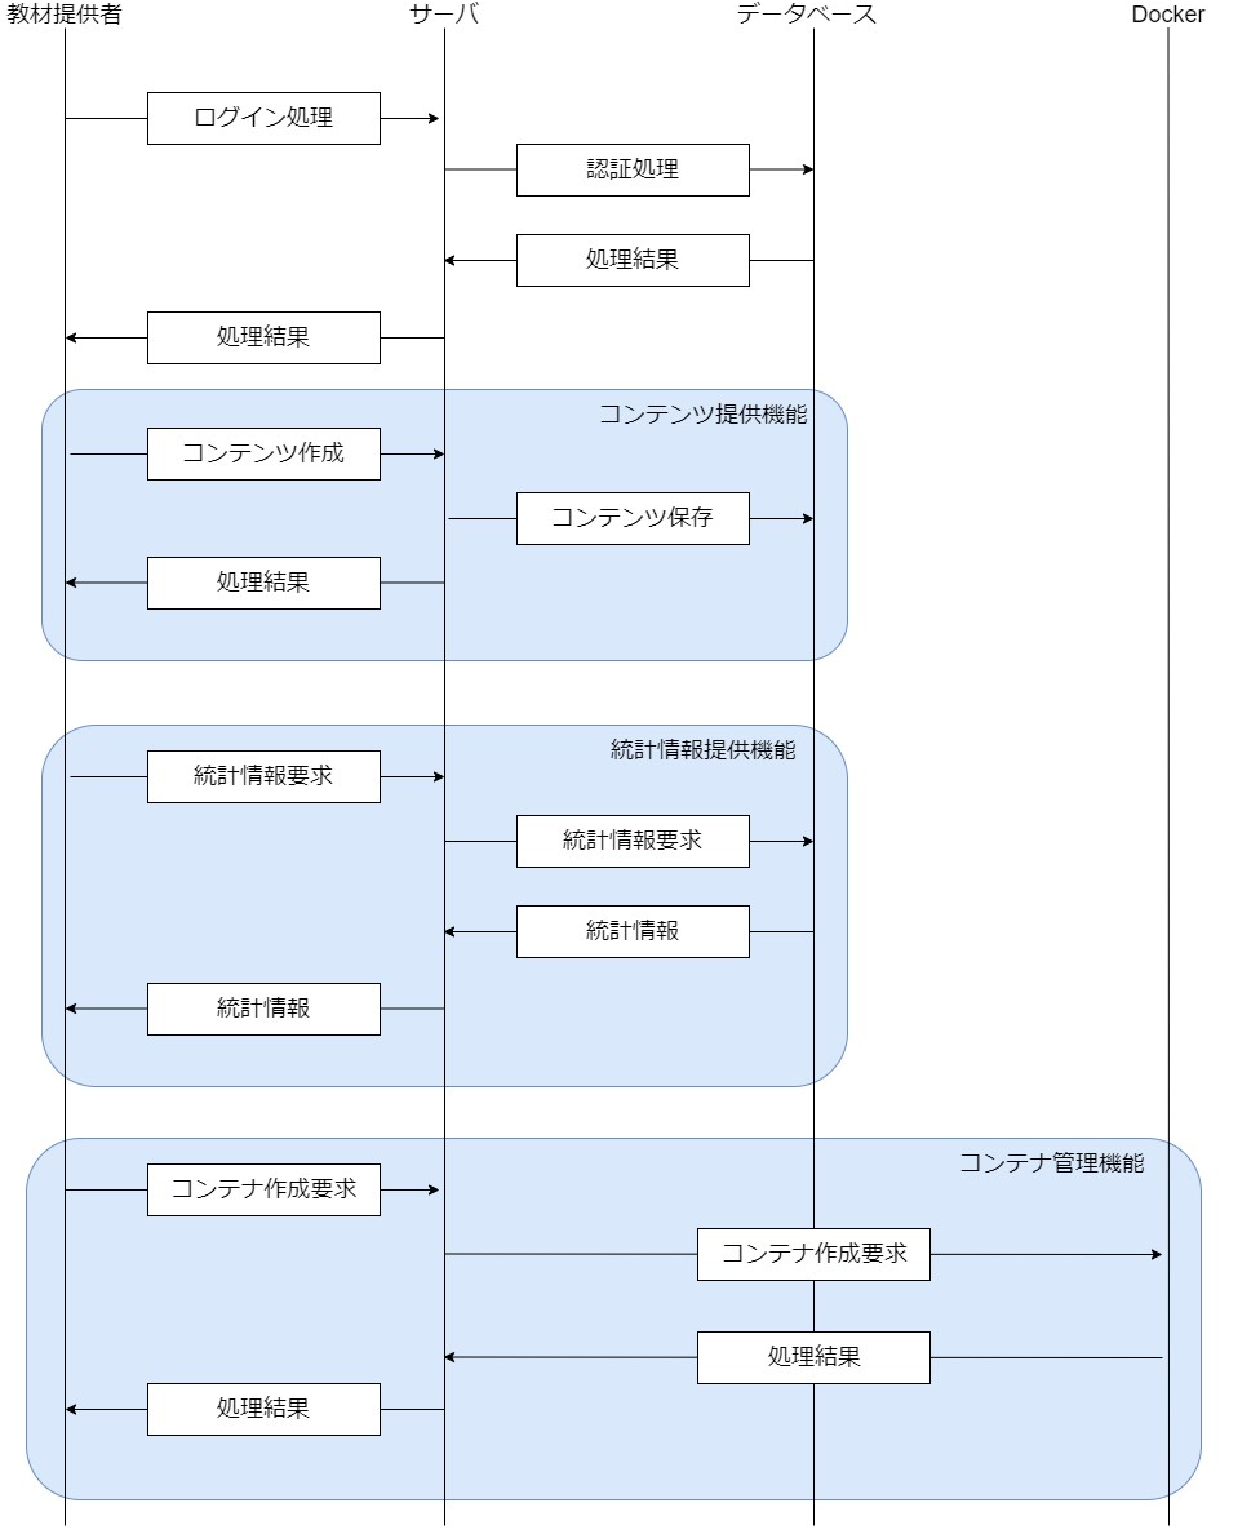
\includegraphics[width=15cm,height=14cm,keepaspectratio]{provider_flow-crop.pdf}\\
        %includegraphicsの詳しい使い方ははLaTeXの参考書を参照.
    \end{center}
    \caption{教材提供者のフローチャート}
    \label{provider_flow}
\end{figure}

\newpage
続いて学習者について説明する.学習者はWebブラウザで本プラットフォームに接続した後,本プラットフォームでアカウント作成できる.アカウント作成には,本プラットフォーム上で表示される
ユーザ名,性別,年齢,パスワードと確認用パスワードが必要である.アカウント作成後,トップページにて教材提供者が作成したコンテンツを選択,閲覧できる.

\begin{figure}[htbp]
    \begin{center}
        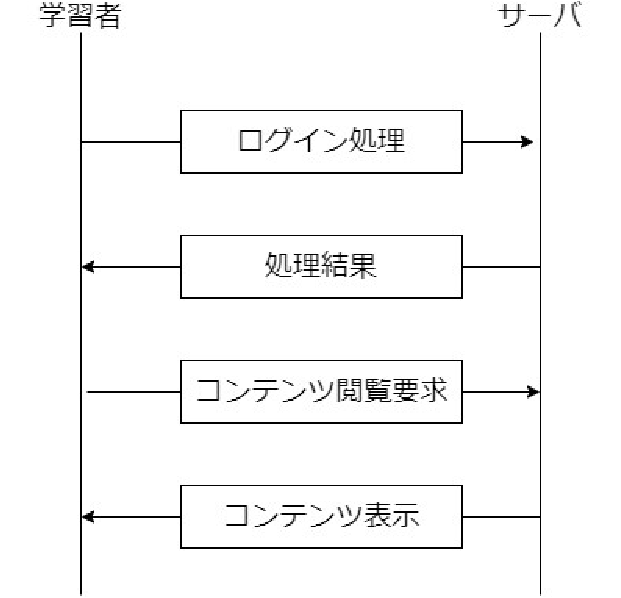
\includegraphics[width=13cm,height=12cm,keepaspectratio]{learn_flow-crop.pdf}\\
        %includegraphicsの詳しい使い方ははLaTeXの参考書を参照.
    \end{center}
    \caption{学習者のフローチャート}
    \label{learn_flow}
\end{figure}

\newpage
\subsection{コンテンツ提供機能}\label{sec:fun1}
日々変化する情報倫理に対応するために,コンテンツを素早く投稿,編集する必要がある.
それに対応するため,教材提供者が情報倫理に関するコンテンツをWebアプリケーション上で提供するためにコンテンツ提供機能を作成した.
本機能ではWeb上で教材提供者のみがコンテンツの投稿と管理ができる.
コンテンツを投稿するときのGUIを図\ref{content_teikyou}に示す.
図\ref{content_teikyou}に示したとおり,コンテンツを投稿するときに必要な情報は,コンテンツのタイトルとコンテンツのタグ,本文である.
本文はマークダウン形式で記入可能であり,画像や動画の挿入が容易にできる.またプレビュー機能もあるため投稿する前にどのような見た目で投稿されるのかを確認できる.

\begin{figure}[htbp]
    \begin{center}
        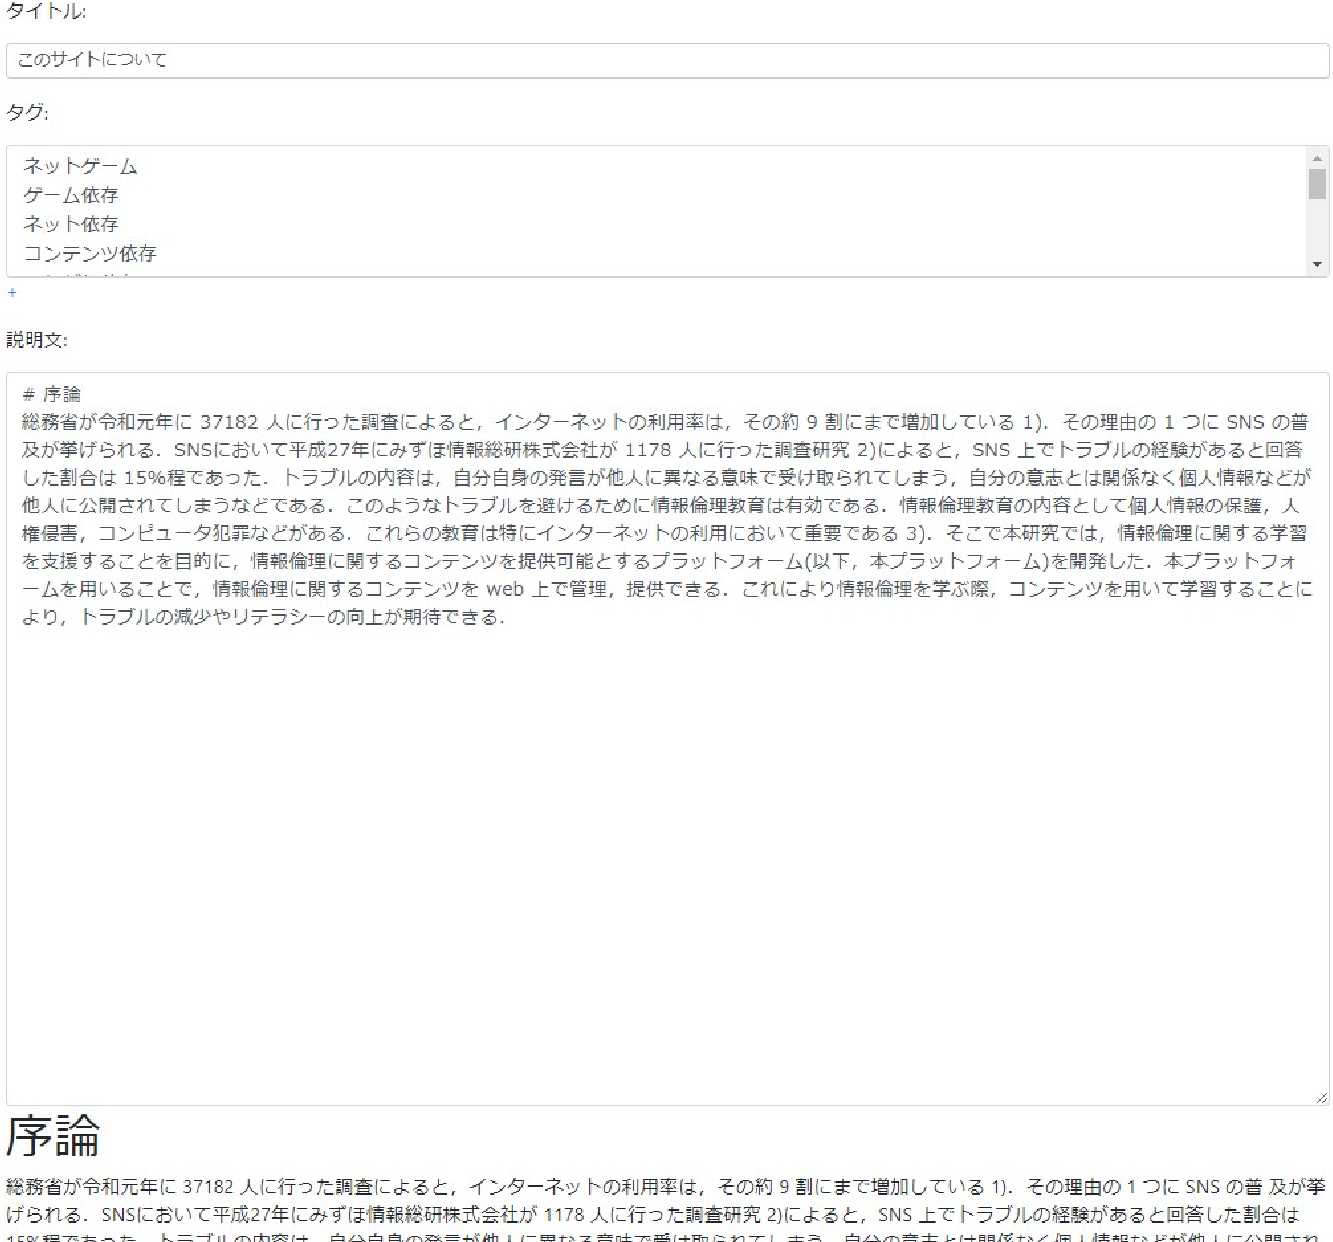
\includegraphics[width=16cm,height=15cm,keepaspectratio]{content_teikyou-crop.pdf}\\
        %includegraphicsの詳しい使い方ははLaTeXの参考書を参照.
    \end{center}
    \caption{コンテンツ提供機能のGUI}
    \label{content_teikyou}
\end{figure}

\newpage
コンテンツのタグは図\ref{content_teikyou}に示すプラスボタンを押下することにより,別画面で新たなタグを登録できる.
タグを登録するときのGUIを図\ref{tag}に示す.
\begin{figure}[htbp]
    \begin{center}
        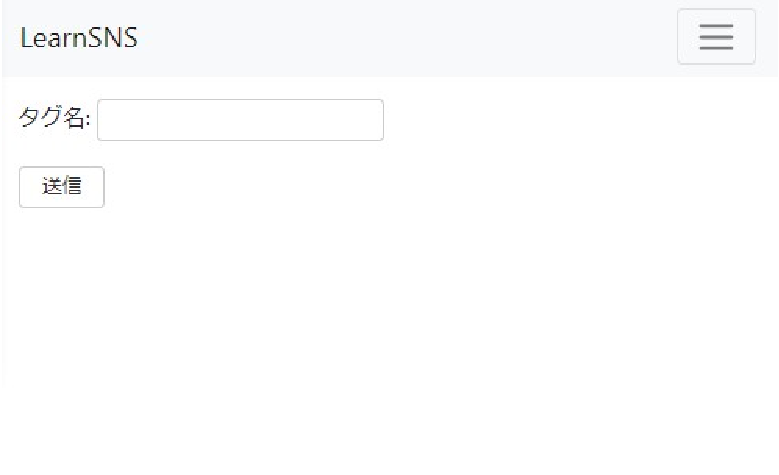
\includegraphics[width=13cm,height=12cm,keepaspectratio]{tag-crop.pdf}\\
        %includegraphicsの詳しい使い方ははLaTeXの参考書を参照.
    \end{center}
    \caption{タグ登録のGUI}
    \label{tag}
\end{figure}

\newpage
また,教材提供者はコンテンツを管理するためのグループに参加する.
そのグループはすべてのコンテンツに対して公開または非公開を選択することでコンテンツを管理する.
グループに参加している教材提供者全員が認可したコンテンツのみが学習者に公開される.
これにより,コンテンツの正当性を担保できる.
教材提供者をグループに参加させるには,図\ref{group_register}のようにして教材提供者のアカウントを選択し教材提供者のグループに登録する.

\begin{figure}[htbp]
    \begin{center}
        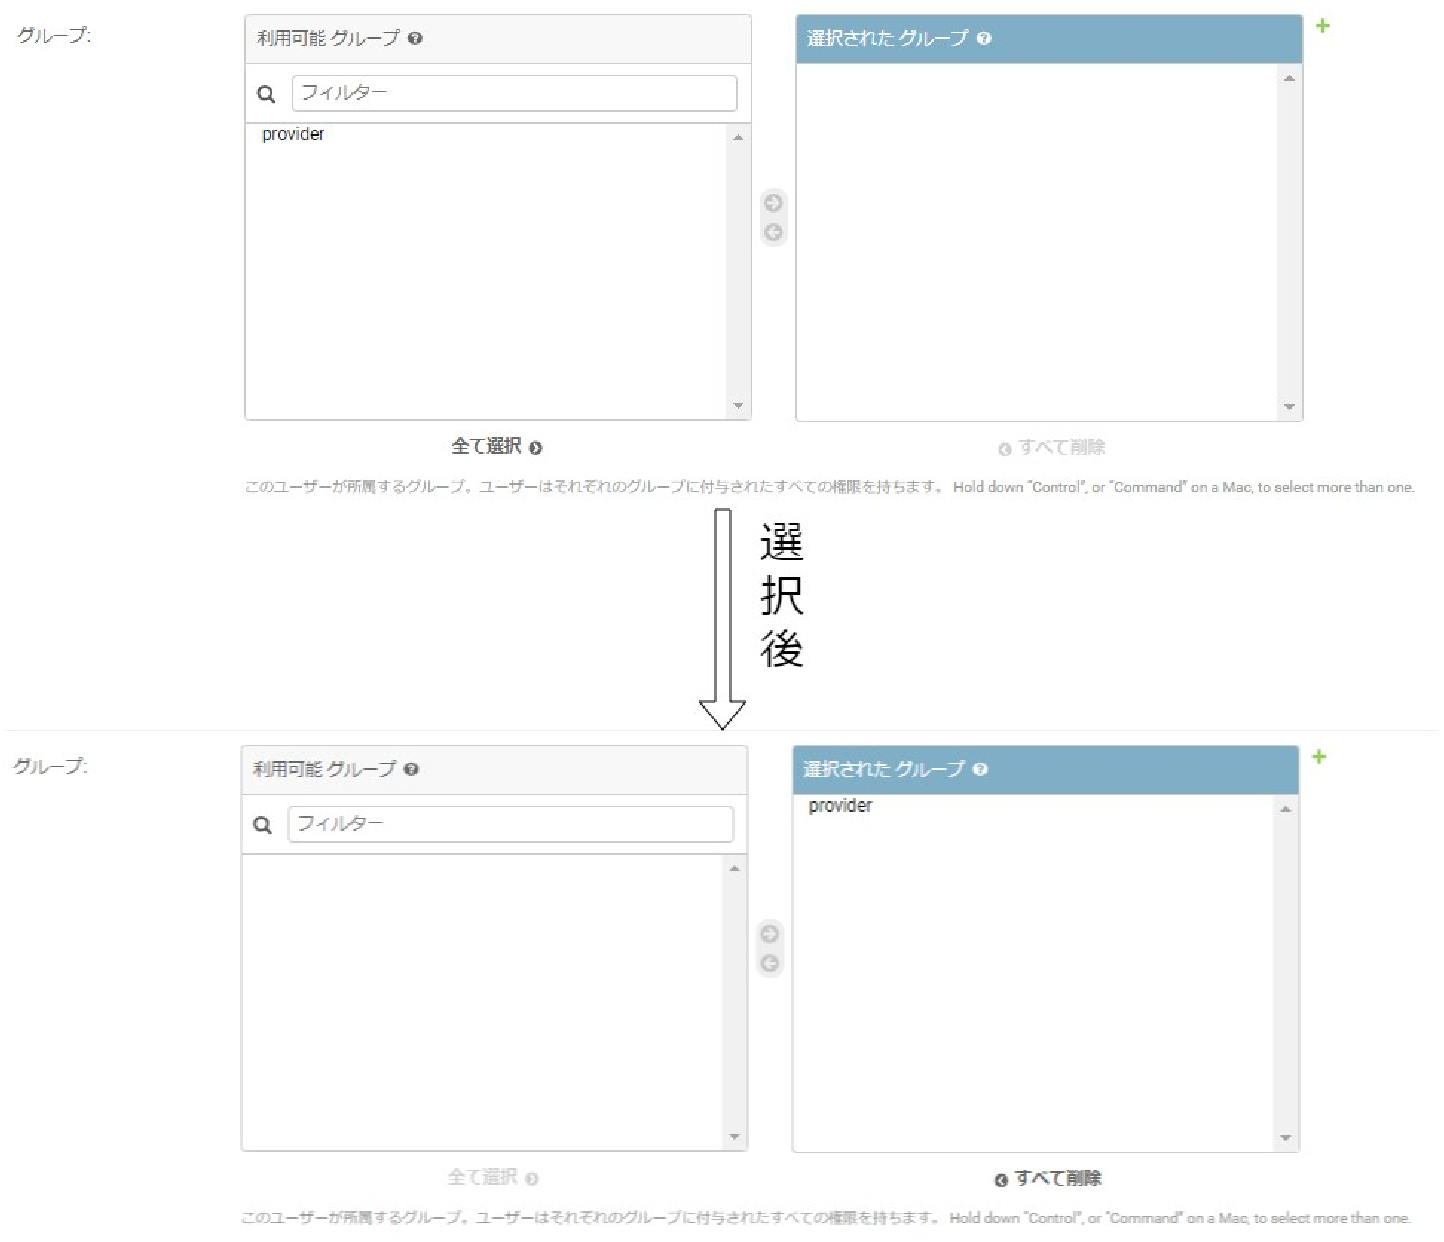
\includegraphics[width=16cm,height=15cm,keepaspectratio]{group_register-crop.pdf}\\
        %includegraphicsの詳しい使い方ははLaTeXの参考書を参照.
    \end{center}
    \caption{グループ登録のGUI}
    \label{group_register}
\end{figure}

\newpage
続いて本機能ではコンテンツ作成後にコンテンツの4択問題を作成することができる.問題の作成には,問題のタイトル,問題文,選択肢1~4および正解の選択肢をフォームに従って入力する.
問題作成時のGUIを図\ref{create_question}に示す.

\begin{figure}[htbp]
    \begin{center}
        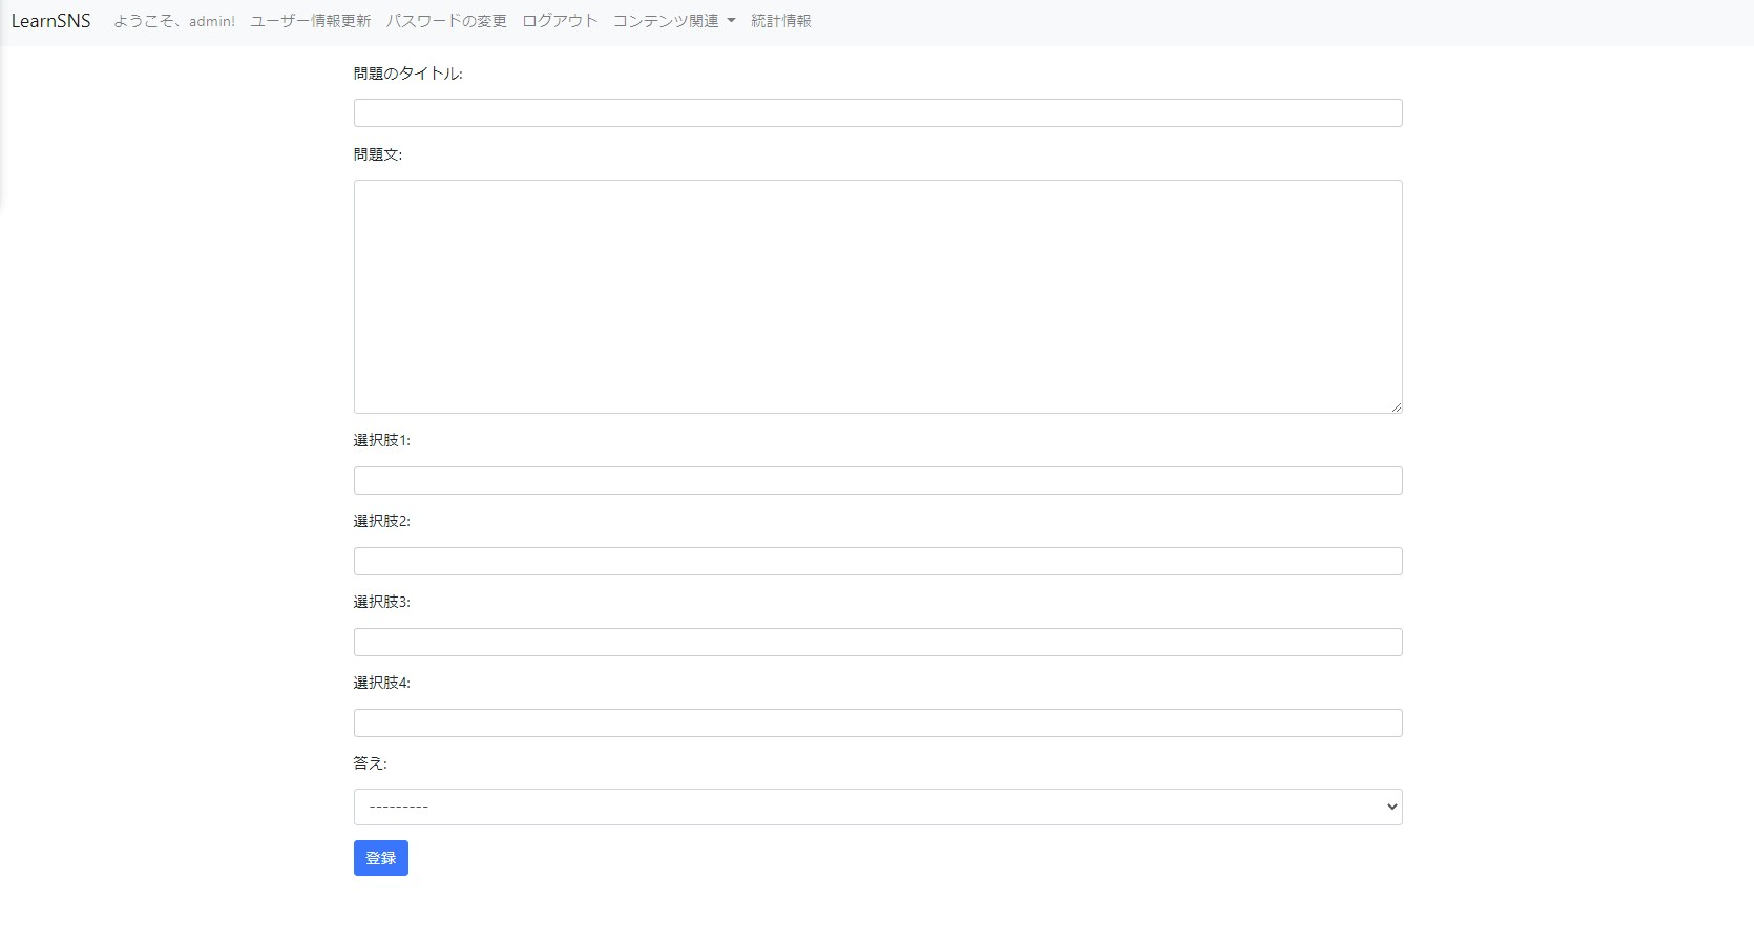
\includegraphics[width=18cm,height=17cm,keepaspectratio]{create_question-crop.pdf}\\
        %includegraphicsの詳しい使い方ははLaTeXの参考書を参照.
    \end{center}
    \caption{問題作成のGUI}
    \label{create_question}
\end{figure}

最後に,Djangoの機能を用いることにより本機能で投稿したコンテンツをJsonファイルに変換することができる.
Jsonファイルに変換するには,以下のような手順を経てコマンドを発行すればよい.
これにより,教材提供者はコンテンツを互いにJsonファイルを介して共有することが可能となる.

\begin{enumerate}
    \item 「docker exec -it コンテナ名 /bin/ash」などとして,本プラットフォームを動作させているコンテナにログインする.
    \item cdコマンドを用いてDjangoによって自動的に生成されたmanage.pyファイルと同階層に移動する.
    \item 「python manage.py dumpdata Jsonファイルに変換したいデータのDBのテーブル名 \textgreater 保存するJsonファイル名.json」を実行後,Jsonファイルが生成される.
\end{enumerate}

\newpage
\subsection{統計情報提供機能}\label{sec:fun2}
統計情報提供機能は,年代,性別の違いから情報倫理に関する意識に違いが生まれていることから\cite{isiki},教材提供者が作成した問題を学習者が解いたときの回答情報を基に,グラフで統計情報を提供する機能である.
これにより,教材提供者は作成したコンテンツの質を向上させることができる.
提示する統計情報の内容としては,問題の各選択肢における割合や回答者の年齢層,性別である.
統計情報提供機能のGUIは図\ref{toukei_ex}の通りである.

\begin{figure}[htbp]
    \begin{center}
        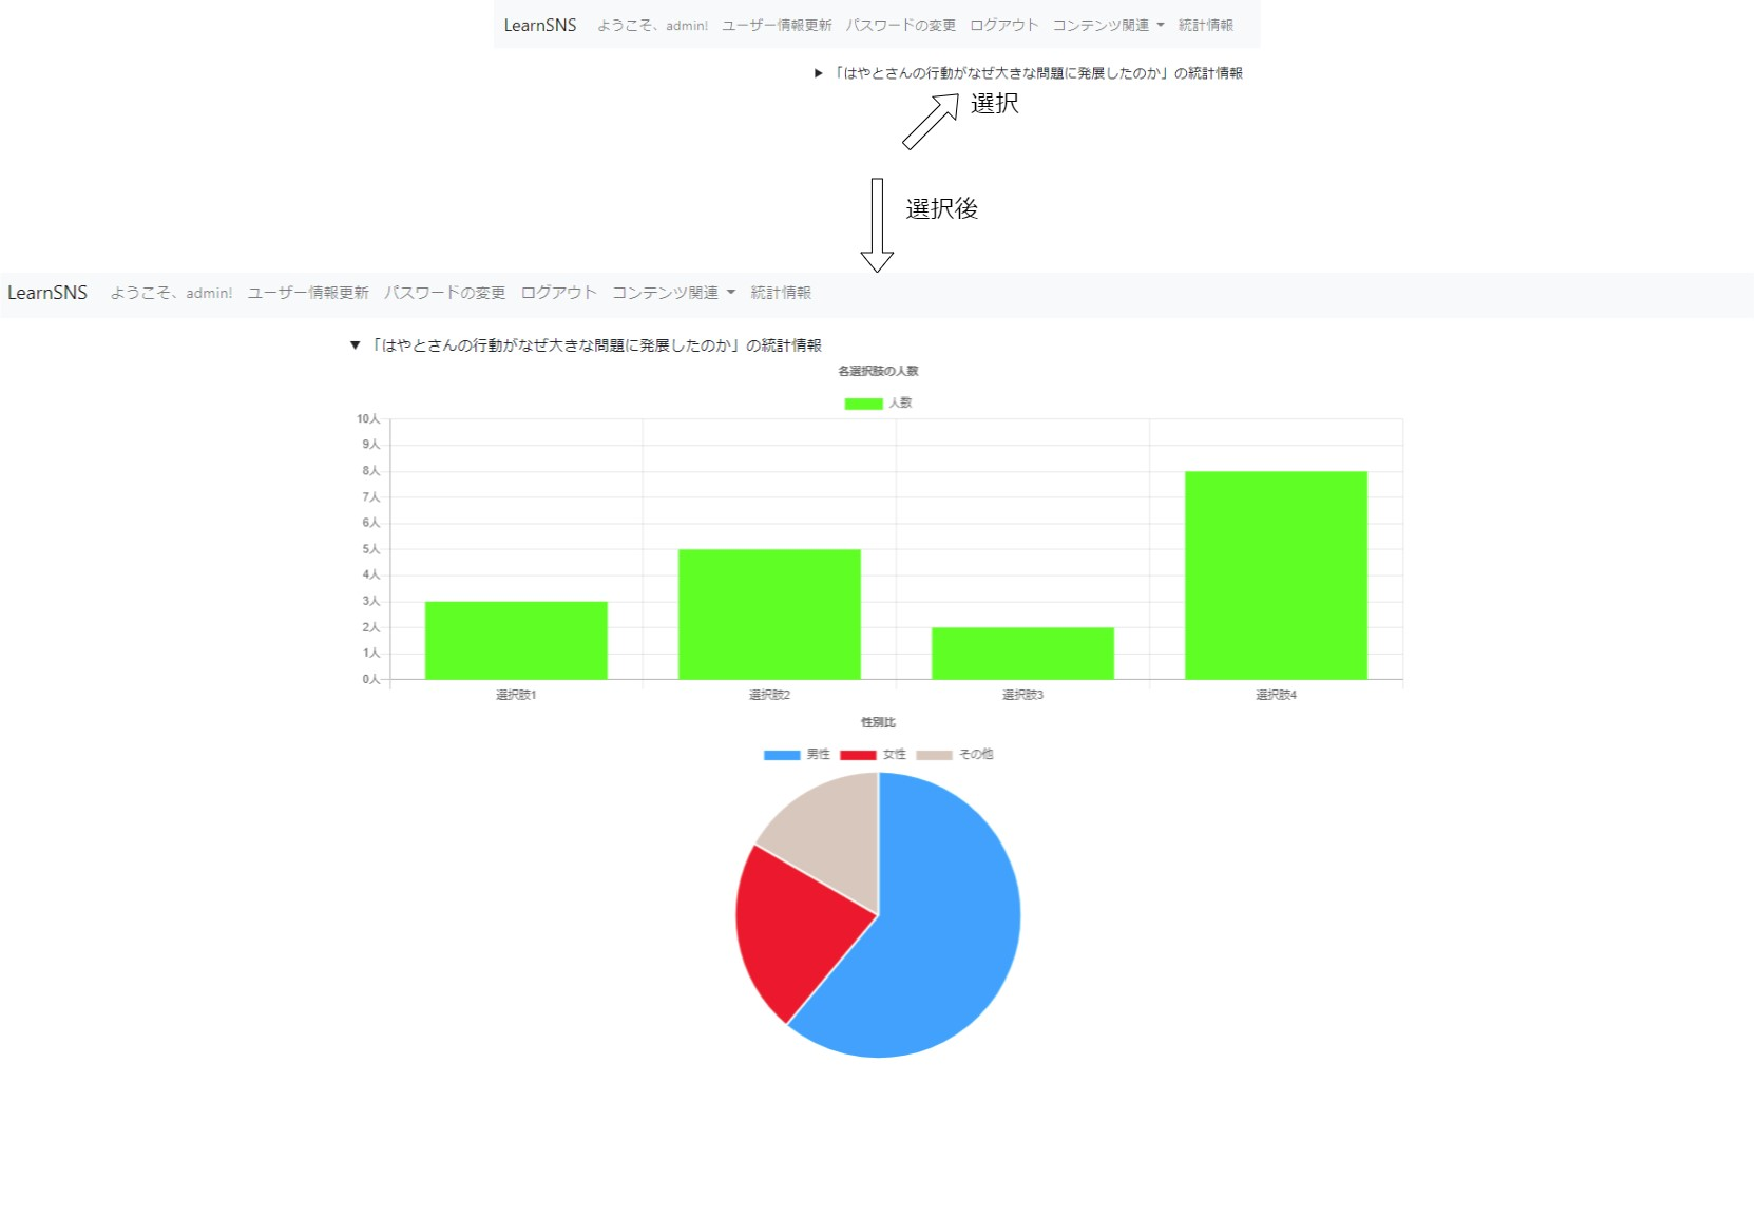
\includegraphics[width=18cm,height=17cm,keepaspectratio]{toukei_ex-crop.pdf}\\
        %includegraphicsの詳しい使い方ははLaTeXの参考書を参照.
    \end{center}
    \caption{統計情報提供機能のGUI}
    \label{toukei_ex}
\end{figure}

\newpage
本機能はChart.jsというjavascriptで作成されたグラフ描画ライブラリを作成している.
Chart.jsでは線グラフ,棒グラフ,レーダーチャート,鶏頭図,ドーナツチャート,円グラフ,バブルチャートを作成できる.
本機能では,棒グラフと円グラフを使用している.

また,本機能で取得可能な情報を表\ref{toukei_info}に示す.
これらの取得できる情報を使って教材提供者はChart.jsで新たなグラフを挿入することができる.

\begin{table}[htb]
    \begin{center}
        \caption{取得可能情報一覧}
            \begin{tabular}{|l|l|} \hline
                取得可能情報 & 詳細 \\ \hline
                学習者情報 &   
                \begin{tabular}{l}
                    年齢\\性別\\回答した問題・選択肢 
                \end{tabular}\\ \hline
                コンテンツ情報 & 問題に対応したコンテンツ \\ \hline
            \end{tabular}
    \label{toukei_info}
    \end{center}
\end{table}

\newpage
\subsection{コンテナ管理機能}\label{sec:fun3}
本プラットフォーム上で,教材提供者は過去のアプリケーションを用いたい場合がある.
それに対応するため,教材提供者がDockerを用いて作成したアプリケーションを本プラットフォームでも利用可能にするためコンテナ管理機能を作成した.
本機能を利用するには,本プラットフォームで動作させたいコンテナ情報が記載されたDockerfileとdocker-compose.ymlを事前にGithubなどのリポジトリに用意する.
外部通信するためのポート番号は,本機能が提示するポート番号のみが利用可能となっている.
以上の情報を,本機能が提示するフォームに入力することにより,本プラットフォームでDockerのコンテナを作成し,アクセスするためのURLが画面上に表示される.
教材提供者は発行されたURLにアクセスすることで動作を確認できる.
また,発行された URL をコンテンツ提供機能の本文に貼り付けることにより,学習者はそのコンテンツを利用できる.

本機能の入力画面と入力が完了し,コンテナが作成された後の画面を図\ref{container_ex_before},図\ref{container_ex_after}に示す.

\begin{figure}[htbp]
    \begin{center}
        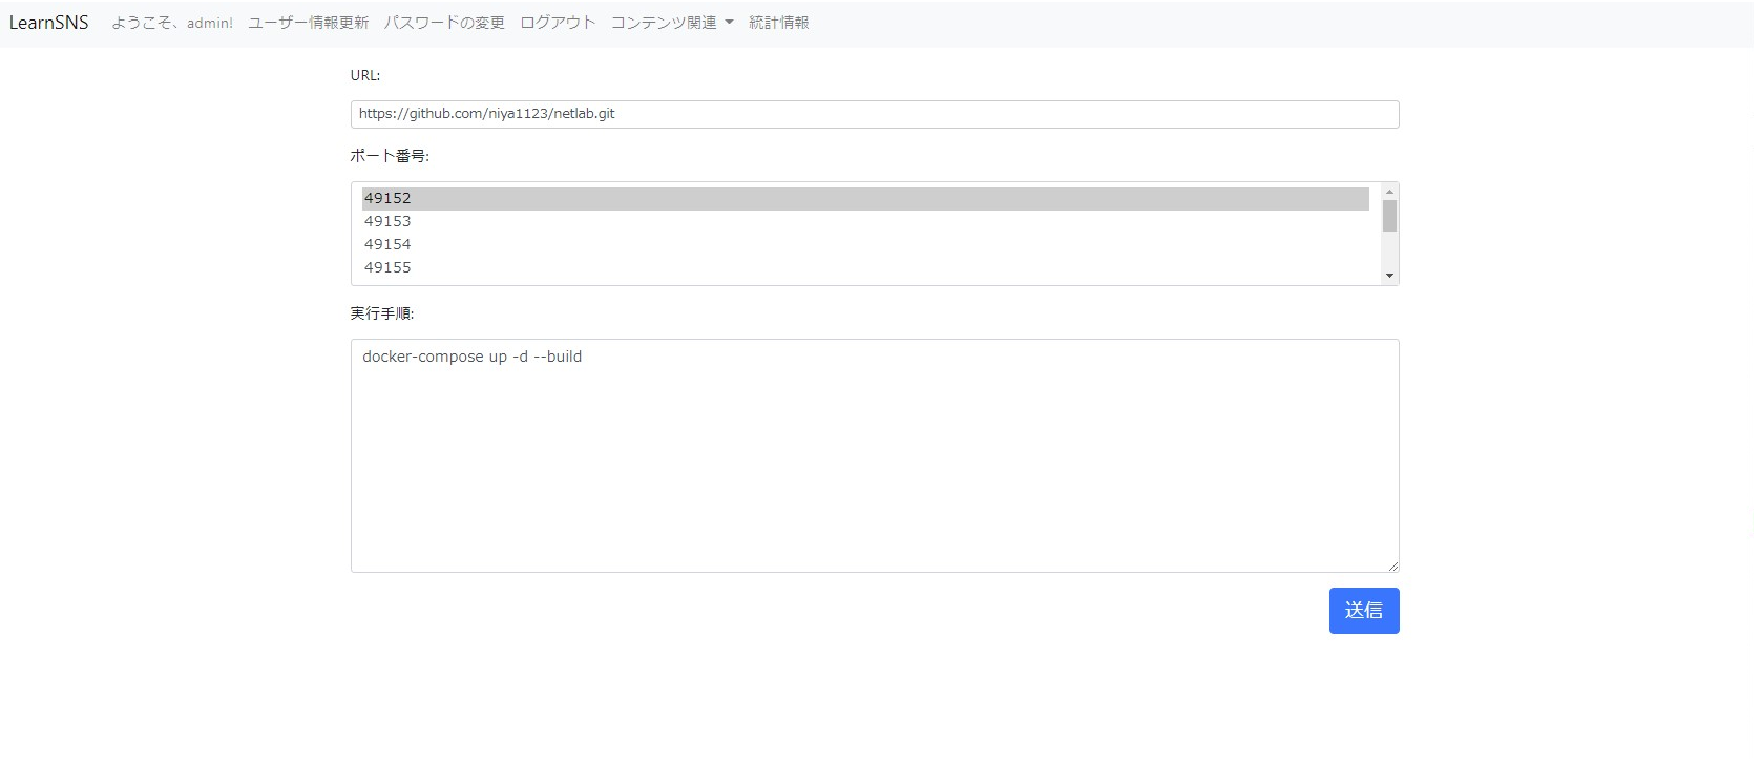
\includegraphics[width=18cm,height=17cm,keepaspectratio]{container_before-crop.pdf}\\
        %includegraphicsの詳しい使い方ははLaTeXの参考書を参照.
    \end{center}
    \caption{コンテナ管理機能の入力画面}
    \label{container_ex_before}
\end{figure}

\begin{figure}[htbp]
    \begin{center}
        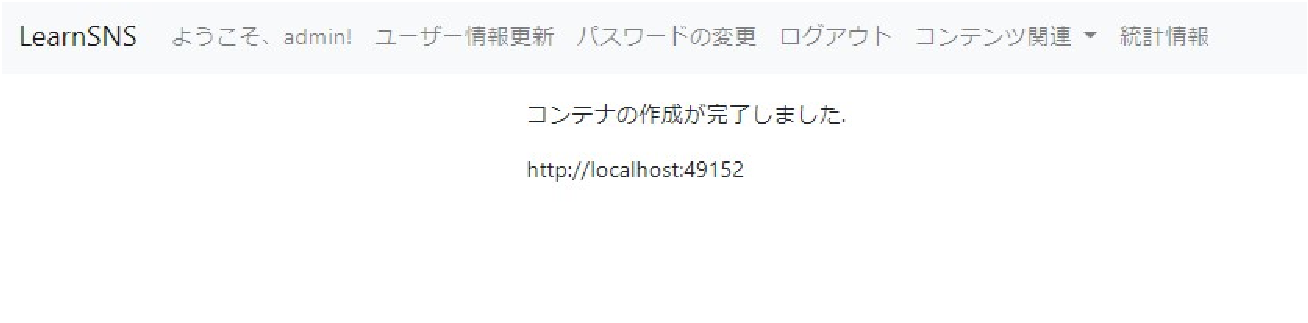
\includegraphics[width=13cm,height=12cm,keepaspectratio]{container_after-crop.pdf}\\
        %includegraphicsの詳しい使い方ははLaTeXの参考書を参照.
    \end{center}
    \caption{コンテナ管理機能のコンテナ作成後の画面}
    \label{container_ex_after}
\end{figure}




%
% 実験・考察
%
\section{実験・考察}\label{se4}

本章では,実施した利用評価実験の内容と結果および考察について述べる.

\subsection{利用評価実験}
本プラットフォームが,学習者に対し情報倫理に関するコンテンツを提供でき,そのコンテンツを見て学ぶことにより情報倫理に関するトラブルの減少とリテラシーの向上が期待できるかどうかを確認するために,利用評価実験を行った.
実験では20代男性10人に対して,本プラットフォームのコンテンツを事前に学習したコンテンツ利用者群と,事前に学習していないコンテンツ非利用者群の5人ずつに分かれて実験を行った.
そして各々の群に対し,GoogleFormを用いて全5問の情報倫理に関する問題を解いてもらった.
ただし,コンテンツ非利用者群に対してGoogleFormで問題を解くときに,わからない単語等があれば調べてもよいとした.

このような条件で実施したコンテンツ利用者群とコンテンツ非利用者群の実験結果を図\ref{result_all},図\ref{result_avg}に示す.
図\ref{result_all}はコンテンツ利用者群とコンテンツ非利用者群の獲得点数を表している.
図\ref{result_avg}はコンテンツ利用者群とコンテンツ非利用者群の獲得点数の平均と標準偏差を表している.

\begin{figure}[htbp]
    \begin{center}
        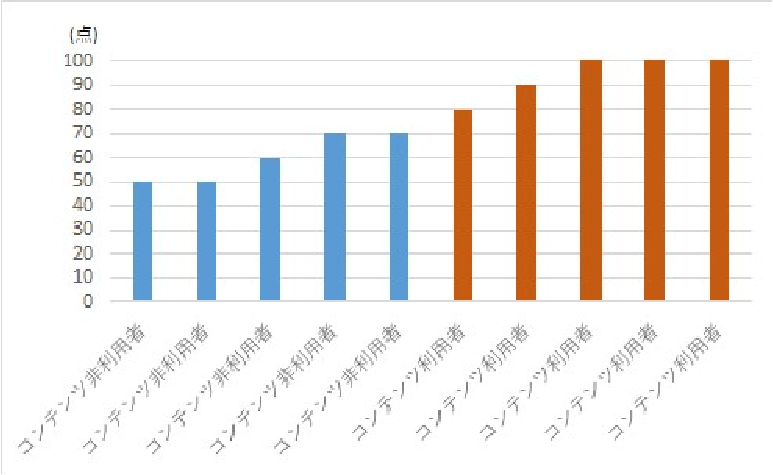
\includegraphics[width=13cm,height=12cm,keepaspectratio]{result_all-crop.pdf}\\
        %includegraphicsの詳しい使い方ははLaTeXの参考書を参照.
    \end{center}
    \caption{コンテンツ利用者群とコンテンツ非利用者群の獲得点数}
    \label{result_all}
\end{figure}
\newpage
\begin{figure}[htbp]
    \begin{center}
        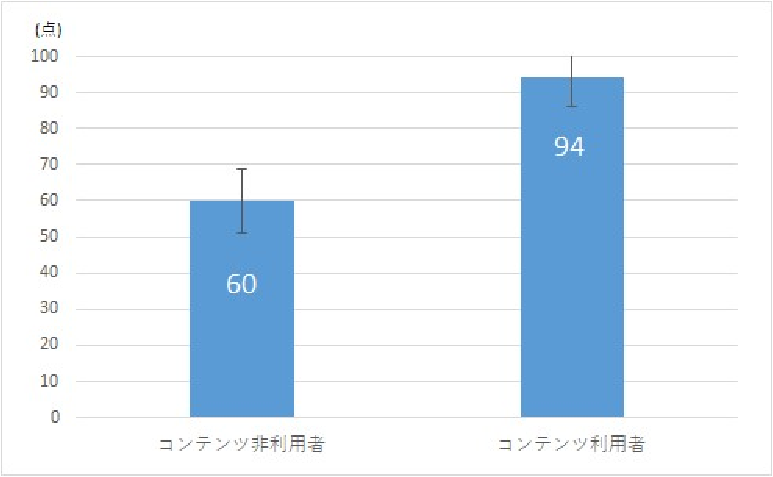
\includegraphics[width=13cm,height=12cm,keepaspectratio]{result-crop.pdf}\\
        %includegraphicsの詳しい使い方ははLaTeXの参考書を参照.
    \end{center}
    \caption{コンテンツ利用者群とコンテンツ非利用者群の獲得点数の平均と標準偏差}
    \label{result_avg}
\end{figure}

実験の結果,平均点においてコンテンツ利用者群が94点,コンテンツ非利用者群が60点と34点の差がついていることが分かった.
また,標準偏差においてはコンテンツ利用者群が 8.00,コンテンツ非利用者群が 8.94 であり,0.94 の差がついている.
以上から,本プラットフォームを用いて情報倫理について学習すると,点数のばらつきはコンテンツ利用者群の方がなく,点数も平均点の差からコンテンツ非利用者群と比べ高くなっていることがわかる.
このことからコンテンツ非利用者群は,情婦倫理に関して単語の記憶,理解だけを行っておりその結果情報倫理に対して十分な理解を得られずに問題を解き点数が低くなったと考えられる.
一方,コンテンツ利用者群は,本プラットフォームで提示したコンテンツを学んでいる.このコンテンツには実際に起こりうる情報倫理に関する問題をシナリオ形式で提示している.
このことによりコンテンツ利用者群は情報倫理に関して深く理解を得られたのではないかと考えられる.
したがって,本プラットフォームは学習者に対して,情報倫理に関するトラブルの減少とリテラシー向上を期待できる.


%
% 結論・今後の課題
%
\section{結論・今後の課題}\label{sec5}
本研究では,持続的な学習環境を提供することを目的に,情報倫理教育におけるeラーニングのためのプラットフォームを開発する.
まず,本稿ではコンテンツの作成,統計情報の確認,外部アプリケーションの導入を補佐する機能を開発した.
本プラットフォームを用いることで,情報倫理に関するコンテンツを web 上で管理,提供でき,持続的にコンテンツの提供ができる.
これらのコンテンツを用いて学習することにより,トラブルの減少やリテラシーの理解を期待できる.

今後の予定として,教育効果を高めると言われるアニメーションを利用し\cite{elsec},本プラットフォーム上で情報倫理に関するアニメーション作成の支援が行えるような機能を作成する予定である.


%
% 謝辞
%
本論文は近畿大学大学院総合理工学研究科エレクトロニクス系工学専攻においての研究成果をまとめたものである.

本研究を遂行するに当たり,熱心な御指導および御鞭撻をいただきました指導教員である近畿大学情報学部の井口信和教授,近畿大学情報学部の越智洋司准教授,近畿大学情報学部の山元翔講師に深く感謝の意を表します.

論文審査にあたり,主査を担当して下さいました近畿大学情報学部の越智洋司准教授,副主査を担当して下さいました近畿大学情報学部の森山真光准教授に心より御礼申し上げます.

%
% 参考文献
%
\bibliography{references} %references.bibから拡張子を外した名前
\bibliographystyle{junsrt} %参考文献出力スタイル

%
% 付録
%
% \appendix
\section{付録について}
本研究で作成したプログラムのソースファイルなどを卒業研究報告書に含めた
い場合は,付録として巻末にまとめておく.

\end{document}